% Options for packages loaded elsewhere
\PassOptionsToPackage{unicode}{hyperref}
\PassOptionsToPackage{hyphens}{url}
\PassOptionsToPackage{dvipsnames,svgnames,x11names}{xcolor}
%
\documentclass[
]{krantz}
\title{Crime by the Numbers: A Criminologist's Guide to R}
\author{Jacob Kaplan}
\date{2022-01-24}

\usepackage{amsmath,amssymb}
\usepackage{lmodern}
\usepackage{iftex}
\ifPDFTeX
  \usepackage[T1]{fontenc}
  \usepackage[utf8]{inputenc}
  \usepackage{textcomp} % provide euro and other symbols
\else % if luatex or xetex
  \usepackage{unicode-math}
  \defaultfontfeatures{Scale=MatchLowercase}
  \defaultfontfeatures[\rmfamily]{Ligatures=TeX,Scale=1}
  \setmonofont[Scale=0.7]{Source Code Pro}
\fi
% Use upquote if available, for straight quotes in verbatim environments
\IfFileExists{upquote.sty}{\usepackage{upquote}}{}
\IfFileExists{microtype.sty}{% use microtype if available
  \usepackage[]{microtype}
  \UseMicrotypeSet[protrusion]{basicmath} % disable protrusion for tt fonts
}{}
\makeatletter
\@ifundefined{KOMAClassName}{% if non-KOMA class
  \IfFileExists{parskip.sty}{%
    \usepackage{parskip}
  }{% else
    \setlength{\parindent}{0pt}
    \setlength{\parskip}{6pt plus 2pt minus 1pt}}
}{% if KOMA class
  \KOMAoptions{parskip=half}}
\makeatother
\usepackage{xcolor}
\IfFileExists{xurl.sty}{\usepackage{xurl}}{} % add URL line breaks if available
\IfFileExists{bookmark.sty}{\usepackage{bookmark}}{\usepackage{hyperref}}
\hypersetup{
  pdftitle={Crime by the Numbers: A Criminologist's Guide to R},
  pdfauthor={Jacob Kaplan},
  colorlinks=true,
  linkcolor={Maroon},
  filecolor={Maroon},
  citecolor={Blue},
  urlcolor={Blue},
  pdfcreator={LaTeX via pandoc}}
\urlstyle{same} % disable monospaced font for URLs
\usepackage{color}
\usepackage{fancyvrb}
\newcommand{\VerbBar}{|}
\newcommand{\VERB}{\Verb[commandchars=\\\{\}]}
\DefineVerbatimEnvironment{Highlighting}{Verbatim}{commandchars=\\\{\}}
% Add ',fontsize=\small' for more characters per line
\usepackage{framed}
\definecolor{shadecolor}{RGB}{248,248,248}
\newenvironment{Shaded}{\begin{snugshade}}{\end{snugshade}}
\newcommand{\AlertTok}[1]{\textcolor[rgb]{0.94,0.16,0.16}{#1}}
\newcommand{\AnnotationTok}[1]{\textcolor[rgb]{0.56,0.35,0.01}{\textbf{\textit{#1}}}}
\newcommand{\AttributeTok}[1]{\textcolor[rgb]{0.77,0.63,0.00}{#1}}
\newcommand{\BaseNTok}[1]{\textcolor[rgb]{0.00,0.00,0.81}{#1}}
\newcommand{\BuiltInTok}[1]{#1}
\newcommand{\CharTok}[1]{\textcolor[rgb]{0.31,0.60,0.02}{#1}}
\newcommand{\CommentTok}[1]{\textcolor[rgb]{0.56,0.35,0.01}{\textit{#1}}}
\newcommand{\CommentVarTok}[1]{\textcolor[rgb]{0.56,0.35,0.01}{\textbf{\textit{#1}}}}
\newcommand{\ConstantTok}[1]{\textcolor[rgb]{0.00,0.00,0.00}{#1}}
\newcommand{\ControlFlowTok}[1]{\textcolor[rgb]{0.13,0.29,0.53}{\textbf{#1}}}
\newcommand{\DataTypeTok}[1]{\textcolor[rgb]{0.13,0.29,0.53}{#1}}
\newcommand{\DecValTok}[1]{\textcolor[rgb]{0.00,0.00,0.81}{#1}}
\newcommand{\DocumentationTok}[1]{\textcolor[rgb]{0.56,0.35,0.01}{\textbf{\textit{#1}}}}
\newcommand{\ErrorTok}[1]{\textcolor[rgb]{0.64,0.00,0.00}{\textbf{#1}}}
\newcommand{\ExtensionTok}[1]{#1}
\newcommand{\FloatTok}[1]{\textcolor[rgb]{0.00,0.00,0.81}{#1}}
\newcommand{\FunctionTok}[1]{\textcolor[rgb]{0.00,0.00,0.00}{#1}}
\newcommand{\ImportTok}[1]{#1}
\newcommand{\InformationTok}[1]{\textcolor[rgb]{0.56,0.35,0.01}{\textbf{\textit{#1}}}}
\newcommand{\KeywordTok}[1]{\textcolor[rgb]{0.13,0.29,0.53}{\textbf{#1}}}
\newcommand{\NormalTok}[1]{#1}
\newcommand{\OperatorTok}[1]{\textcolor[rgb]{0.81,0.36,0.00}{\textbf{#1}}}
\newcommand{\OtherTok}[1]{\textcolor[rgb]{0.56,0.35,0.01}{#1}}
\newcommand{\PreprocessorTok}[1]{\textcolor[rgb]{0.56,0.35,0.01}{\textit{#1}}}
\newcommand{\RegionMarkerTok}[1]{#1}
\newcommand{\SpecialCharTok}[1]{\textcolor[rgb]{0.00,0.00,0.00}{#1}}
\newcommand{\SpecialStringTok}[1]{\textcolor[rgb]{0.31,0.60,0.02}{#1}}
\newcommand{\StringTok}[1]{\textcolor[rgb]{0.31,0.60,0.02}{#1}}
\newcommand{\VariableTok}[1]{\textcolor[rgb]{0.00,0.00,0.00}{#1}}
\newcommand{\VerbatimStringTok}[1]{\textcolor[rgb]{0.31,0.60,0.02}{#1}}
\newcommand{\WarningTok}[1]{\textcolor[rgb]{0.56,0.35,0.01}{\textbf{\textit{#1}}}}
\usepackage{longtable,booktabs,array}
\usepackage{calc} % for calculating minipage widths
% Correct order of tables after \paragraph or \subparagraph
\usepackage{etoolbox}
\makeatletter
\patchcmd\longtable{\par}{\if@noskipsec\mbox{}\fi\par}{}{}
\makeatother
% Allow footnotes in longtable head/foot
\IfFileExists{footnotehyper.sty}{\usepackage{footnotehyper}}{\usepackage{footnote}}
\makesavenoteenv{longtable}
\usepackage{graphicx}
\makeatletter
\def\maxwidth{\ifdim\Gin@nat@width>\linewidth\linewidth\else\Gin@nat@width\fi}
\def\maxheight{\ifdim\Gin@nat@height>\textheight\textheight\else\Gin@nat@height\fi}
\makeatother
% Scale images if necessary, so that they will not overflow the page
% margins by default, and it is still possible to overwrite the defaults
% using explicit options in \includegraphics[width, height, ...]{}
\setkeys{Gin}{width=\maxwidth,height=\maxheight,keepaspectratio}
% Set default figure placement to htbp
\makeatletter
\def\fps@figure{htbp}
\makeatother
\setlength{\emergencystretch}{3em} % prevent overfull lines
\providecommand{\tightlist}{%
  \setlength{\itemsep}{0pt}\setlength{\parskip}{0pt}}
\setcounter{secnumdepth}{5}
\usepackage{booktabs}
\usepackage{longtable}
\usepackage[bf,singlelinecheck=off]{caption}
\usepackage{emptypage}
\usepackage[T1]{fontenc}
\usepackage{lmodern}
\usepackage{listings} \let\verbatim\undefined \let\verbatimend\undefined \lstnewenvironment{verbatim}{\lstset{breaklines,basicstyle=\ttfamily}}{}
\usepackage{framed,color}
\definecolor{shadecolor}{RGB}{248,248,248}

\usepackage{float}
\let\origfigure\figure
\let\endorigfigure\endfigure
\renewenvironment{figure}[1][2] {
    \expandafter\origfigure\expandafter[H]
} {
    \endorigfigure
}
\floatplacement{figure}{H}

\renewcommand{\textfraction}{0.05}
\renewcommand{\topfraction}{0.8}
\renewcommand{\bottomfraction}{0.8}
\renewcommand{\floatpagefraction}{0.75}

\renewenvironment{quote}{\begin{VF}}{\end{VF}}
\let\oldhref\href
\renewcommand{\href}[2]{#2\footnote{\url{#1}}}

\ifxetex
  \usepackage{letltxmacro}
  \setlength{\XeTeXLinkMargin}{1pt}
  \LetLtxMacro\SavedIncludeGraphics\includegraphics
  \def\includegraphics#1#{% #1 catches optional stuff (star/opt. arg.)
    \IncludeGraphicsAux{#1}%
  }%
  \newcommand*{\IncludeGraphicsAux}[2]{%
    \XeTeXLinkBox{%
      \SavedIncludeGraphics#1{#2}%
    }%
  }%
\fi

\makeatletter
\newenvironment{kframe}{%
\medskip{}
\setlength{\fboxsep}{.8em}
 \def\at@end@of@kframe{}%
 \ifinner\ifhmode%
  \def\at@end@of@kframe{\end{minipage}}%
  \begin{minipage}{\columnwidth}%
 \fi\fi%
 \def\FrameCommand##1{\hskip\@totalleftmargin \hskip-\fboxsep
 \colorbox{shadecolor}{##1}\hskip-\fboxsep
     % There is no \\@totalrightmargin, so:
     \hskip-\linewidth \hskip-\@totalleftmargin \hskip\columnwidth}%
 \MakeFramed {\advance\hsize-\width
   \@totalleftmargin\z@ \linewidth\hsize
   \@setminipage}}%
 {\par\unskip\endMakeFramed%
 \at@end@of@kframe}
\makeatother

\renewenvironment{Shaded}{\begin{kframe}}{\end{kframe}}

\usepackage{makeidx}
\makeindex

\urlstyle{tt}

\usepackage{amsthm}
\makeatletter
\def\thm@space@setup{%
  \thm@preskip=8pt plus 2pt minus 4pt
  \thm@postskip=\thm@preskip
}



\makeatother

\frontmatter
\usepackage{float}
\ifLuaTeX
  \usepackage{selnolig}  % disable illegal ligatures
\fi
\usepackage[]{natbib}
\bibliographystyle{apalike}

\begin{document}
\maketitle

%\cleardoublepage\newpage\thispagestyle{empty}\null
%\cleardoublepage\newpage\thispagestyle{empty}\null
%\cleardoublepage\newpage
\thispagestyle{empty}
\begin{center}
To my love Kristina, and our puppies Peanut and Moose.
\end{center}

\setlength{\abovedisplayskip}{-5pt}
\setlength{\abovedisplayshortskip}{-5pt}

{
\hypersetup{linkcolor=}
\setcounter{tocdepth}{2}
\tableofcontents
}
\pagenumbering{roman}

\hypertarget{part-introduction}{%
\chapter*{(PART) Introduction}\label{part-introduction}}
\addcontentsline{toc}{chapter}{(PART) Introduction}

\hypertarget{preface}{%
\chapter*{Preface}\label{preface}}
\addcontentsline{toc}{chapter}{Preface}

This book introduces the programming language R and is meant
for undergrads or graduate students studying criminology. R
is a programming language that is well-suited to the type of
work frequently done in criminology - taking messy data and
turning it into useful information. While R is a useful tool
for many fields of study, this book focuses on the skills
criminologists should know and uses crime data for the
example data sets.

For this book you should have the latest version of
\href{https://cloud.r-project.org/}{R} installed and be
running it through
\href{https://www.rstudio.com/products/rstudio/download/}{RStudio
Desktop (The free version)}. We'll get into detail on what R
and RStudio are soon but please have them both installed to
be able to follow along with each chapter. While you must
install both, you only ever need to open RStudio. While R is
the actual programming language, RStudio is program that
makes it a lot easier to interact with R than opening up the
R application itself.\footnote{This is formally known as an
  ``integrated development environment'' or an IDE.} I
highly recommend following along with the code for each
lesson and then trying to use the lessons learned on a data
set that you are interested in.

\hypertarget{why-learn-to-program}{%
\section*{Why learn to
program?}\label{why-learn-to-program}}
\addcontentsline{toc}{section}{Why learn to program?}

With the exception of some more advanced techniques like
scraping data from websites or from PDFs, nearly everything
we do here can be done through Excel, a software you're
probably more familiar with. The basic steps for research
projects are generally:

\begin{enumerate}
\def\labelenumi{\arabic{enumi}.}
\tightlist
\item
  Open up a data set - which frequently comes as an Excel
  file!
\item
  Change some values - misspellings or too specific
  categories for our purposes are very common in crime data
\item
  Delete some values - such as states you won't be studying
\item
  Make some graphs
\item
  Calculate some values - such as number of crimes per year
\item
  Sometimes do a statistical analysis depending on the type
  of project
\item
  Write up what you find
\end{enumerate}

R can do all of this but why should you want (or have) to
learn an entirely new skill just to do something you can
already do? R is useful for two main reasons: scale and
reproducibility.

\hypertarget{scale}{%
\subsection*{Scale}\label{scale}}
\addcontentsline{toc}{subsection}{Scale}

If you do a one-off project in your career such as
downloading some data and making a graph out of it, it makes
sense to stick with software like Excel. The cost (in time
and effort) of learning R is certainly not worth it for a
single (or even several) project - even one perfectly suited
for using R. R (and many programming languages more
generally, such as Python) has its strength in doing
something fairly simple many times. For example, it may be
quicker to download one file yourself than it is to write
the code in R to download that file. But when it comes to
downloading hundreds of files, writing the R code becomes
very quickly the better option than doing it by hand.

For most tasks you do in research when dealing with data,
you will end up doing them many times (including doing the
same task in future projects). So R offers the trade-off of
spending time upfront by learning the code with the benefit
of that code being able to do work at a large scale with
little extra work from you. Please keep in mind this
trade-off - you need to front-load the costs of learning R
for the rewards of making your life easier when dealing with
data - when feeling discouraged about the small returns you
get early in learning R.

\hypertarget{reproducibility}{%
\subsection*{Reproducibility}\label{reproducibility}}
\addcontentsline{toc}{subsection}{Reproducibility}

The second major benefit of using R over something like
Excel is that R is reproducible. Every action you take is
written down. This is useful when collaborating with others
(including your future self) as they can look at your code
and follow along what you did without you having to show
them every click you made as you frequently would on Excel.
Your collaborator can look at your code to help you figure
out a bug in the code or add their own code to yours.

In the research context specifically, you want to have code
to give to people to ensure that your research was done
correctly and there aren't bugs in the code. Additionally,
if you build a tool to, for example, interpret raw crime
data from an agency and turn it into a map, being able to
share the code so others can modify it for their own city
saves these people a lot of time and effort.

While not required (yet) in criminology, some academic
journals (such as in economics) even require that you submit
your data and code if your paper is accepted. If criminology
follows in this trend, or if you submit to journals that
require code submissions, you'll need to be able to write
code and not rely on software that doesn't track your steps
(such as Excel and SPSS).

\hypertarget{what-you-will-learn}{%
\section*{What you will learn}\label{what-you-will-learn}}
\addcontentsline{toc}{section}{What you will learn}

For many of the lessons we will be working through real
research questions and working from start to finish as you
would on your own project. This involves thinking about what
you want to accomplish from the data you have and what steps
you need to take to reach that goal. This involves more than
just knowing what code to write - it includes figuring out
what your data has, whether it can answer the question
you're asking, and planning out (without writing any code
yet) what you need to do when you start coding. For most
lessons we'll be using actual crime data that is commonly
used in research so you'll become acquainted to a number of
important data sets.

\hypertarget{skills}{%
\subsection*{Skills}\label{skills}}
\addcontentsline{toc}{subsection}{Skills}

There is a large range of skills in criminology research -
far too large to cover in a single book. Here we will
attempt to teach fundamental skills to build a solid
foundation for future work. We'll be focusing on the
following skills and trying to reinforce our skills with
each lesson.

\begin{itemize}
\tightlist
\item
  Subsetting - Taking only certain rows or columns from a
  data set
\item
  Graphing
\item
  Regular expressions - Essentially R's ``Find and Replace''
  function for text
\item
  Getting data from websites (webscraping)
\item
  Getting data from PDFs (PDF scraping)
\item
  Mapping
\item
  Writing documents through R
\end{itemize}

\hypertarget{what-you-wont-learn}{%
\section*{What you won't learn}\label{what-you-wont-learn}}
\addcontentsline{toc}{section}{What you won't learn}

This book is not a statistics book so we will not be
covering any statistical techniques. Though some data sets
we handle are fairly large, this book does not discuss how
to deal with Big Data. While the lessons you learn in this
book can apply to larger data sets, Big Data (which I tend
to define loosely as data that are too large for my computer
to handle) requires special skills that are outside the
realm of this book. If you do intend to deal with huge data
sets I recommend you look at the R package
\href{https://github.com/Rdatatable/data.table/wiki}{data.table}
which is an excellent resource for it. While we briefly
cover mapping, this book will not cover working with
geographic data in detail. For a comprehensive look at
geographic data please see this
\href{https://geocompr.robinlovelace.net/}{book}. This book
also will not cover any qualitative data or analysis. While
qualitative research is an important part of criminology,
this book only focuses on working with quantitative data.
Some parts of this book may apply to dealing with
qualitative data, such as PDF scraping and regular
expressions, but the examples I use in those chapters still
deal with quantitative data.

\hypertarget{simple-vs-easy}{%
\section*{Simple vs Easy}\label{simple-vs-easy}}
\addcontentsline{toc}{section}{Simple vs Easy}

In the course of this book we will cover things that are
very simple. For example, we'll take a data set (think of it
like an Excel file) with crime for nearly every police
agency in the United States and keep only data from Colorado
for a small number of years. We'll then find out how many
murders happened in Colorado each year. This is a fairly
simple task - it can be expressed in two sentences. You'll
find that most of what you do is simple like this - it is
quick to talk about what you are doing and the concepts are
not complicated. What it isn't is easy. To actually write
the R code to do this takes knowing a number of interrelated
concepts in R and several lines of code to implement each
step.

While this distinction may seem minor, I think it is
important for newer programmers to understand that what they
are doing may be simple to talk about but hard to implement.
It is easy to feel like a bad programmer because something
that can be articulated in 10 seconds may take hours to do.
So during times when you are working with R try to keep in
mind that even though a project may be simple to articulate,
it may be hard to code and that there is often very little
correlation between the two.

\hypertarget{how-to-read-this-book}{%
\section*{How to read this
book}\label{how-to-read-this-book}}
\addcontentsline{toc}{section}{How to read this book}

This book is written so a person who has no programming
experience can start with this chapter and by the end of the
book be able to do a data project from start to finish. Each
chapter introduces a new skill and builds on the skills
introduced in previous chapters. So if you skip ahead you
may miss important skills taught in the chapters you didn't
read. For someone who has no - or minimal - programming
experience, I recommend reading each chapter in order. If
you have more programming experience and just want to learn
how to do a specific thing, feel free to skip directly to
that chapter.

\hypertarget{citing-this-book}{%
\section*{Citing this book}\label{citing-this-book}}
\addcontentsline{toc}{section}{Citing this book}

If this book was useful in your research, please cite it. To
cite this book, please use the below citation:

Kaplan J (2021). \emph{Crime by the Numbers: A
Criminologist's Guide to R}.
\url{https://crimebythenumbers.com/}.

BibTeX format:

\begin{Shaded}
\begin{Highlighting}[]
\VariableTok{@Manual}\NormalTok{\{}\OtherTok{crimebythenumbers}\NormalTok{,}
  \DataTypeTok{title}\NormalTok{ = \{Crime by the Numbers: A Criminologist\textquotesingle{}s Guide to R\},}
  \DataTypeTok{author}\NormalTok{ = \{Jacob Kaplan\},}
  \DataTypeTok{year}\NormalTok{ = \{2021\},}
  \DataTypeTok{url}\NormalTok{ = \{https://crimebythenumbers.com/\},}
\NormalTok{\}}
\end{Highlighting}
\end{Shaded}

\hypertarget{how-to-contribute-to-this-book}{%
\section*{How to contribute to this
book}\label{how-to-contribute-to-this-book}}
\addcontentsline{toc}{section}{How to contribute to this
book}

If you have any questions, suggestions (such as a topic to
cover), or find any issues, please make a post on the
\href{https://github.com/jacobkap/crimebythenumbers/issues}{Issues
page} for this book on GitHub. On this page you can create a
new issue (which is basically just a post on this forum)
with a title and a longer description of your issue. You'll
need a GitHub account to make a post. Posting here lets me
track issues and respond to your message or alert you when
the issue is closed (i.e.~I've finished or denied the
request). Issues are also public so you can see if someone
has already posted something similar.

For more minor issues like typos or grammar mistakes, you
can edit the book directly through its GitHub page. That'll
make an update for me to accept, which will change the book
to include your edit. To do that, click the edit button at
the top of the site - the button is highlighted in the below
figure. You will need to make a GitHub account to make
edits. When you click on that button you'll be taken to a
page that looks like a Word Doc where you can make edits.
Make any edits you want and then scroll to the bottom of the
page. There you can write a short (please, no more than a
sentence or two) description of what you've done and then
submit the changes for me to review.

\begin{center}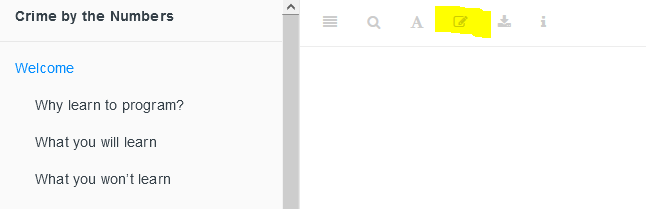
\includegraphics[width=1\linewidth,height=0.45\textheight,]{images/edit_button} \end{center}

Please only use the above two methods to contribute or make
suggestions about the book. Don't email me. While it's a bit
more work for you to do it this way, since you'll need to
make a GitHub account if you don't already have one, it
helps me. I wrote this book, in part, to help my career so
having evidence that people read it and are contributing to
it is important to me. It's a way to publicly measure the
book's impact.

\hypertarget{where-to-find-data-included-in-this-book}{%
\section*{Where to find data included in this
book}\label{where-to-find-data-included-in-this-book}}
\addcontentsline{toc}{section}{Where to find data included
in this book}

To download the data used in this book please see
\href{https://github.com/jacobkap/r4crimz/tree/master/data}{here}.
Each of the files that are used in this book are available
to download at that link. At the top of every chapter that
uses one of these files I'll say exactly which file(s) you
need to download. The best way to use this book is to follow
along by downloading the data and running the code that I
include in each chapter.

\hypertarget{where-to-find-code-included-in-this-book}{%
\section*{Where to find code included in this
book}\label{where-to-find-code-included-in-this-book}}
\addcontentsline{toc}{section}{Where to find code included
in this book}

If you're reading this book through its
\href{https://crimebythenumbers.com}{website} you can easily
copy the code by clicking on the ``Copy to clipboard''
option on the top right of every chunk of code. This button,
shown in the image below, will copy all of the code in the
chunk and you can then paste (through Control/Command+V)
into R.

\begin{center}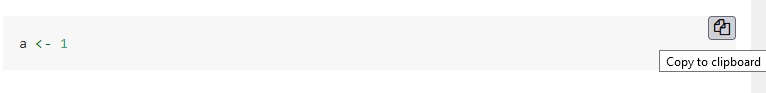
\includegraphics[width=1\linewidth,height=0.45\textheight,]{images/copy_code} \end{center}

I've also made each chapter available to download as an R
file that has every line of code used in each chapter
available to you to run. To download the files, please go to
the book's GitHub page
\href{https://github.com/jacobkap/crimebythenumbers/tree/master/code_repository}{here}.
I've saved each chapter twice - once where it only includes
the code used (in the ``just\_code'' folder) and once where
it includes the code and all of the text in the chapter (in
the ``code\_and\_text'' folder). So download whichever one
you want to use. The code is identical in each.

\hypertarget{interactive-maps}{%
\chapter{Interactive maps}\label{interactive-maps}}

For this chapter you'll need the following files, which are
available for download
\href{https://github.com/jacobkap/r4crimz/tree/master/data}{here}:
san\_francisco\_marijuana\_geocoded.csv and
sf\_neighborhoods\_suicide.rda.

While maps of data are useful, their ability to show
incident-level information is quite limited. They tend to
show broad trends - where crime happened in a city - rather
than provide information about specific crime incidents.
While broad trends are important, there are significant
drawbacks about being unable to get important information
about an incident without having to check the data. An
interactive map bridges this gap by showing trends while
allowing you to zoom into individual incidents and see
information about each incident.

For this lesson we will be using data on every marijuana
dispensary in San Francisco that has an active dispensary
license as of late September 2019. The file is called
``san\_francisco\_marijuana\_geocoded.csv''.

When downloaded from California's Bureau of Cannabis Control
(\href{https://aca5.accela.com/bcc/customization/bcc/cap/licenseSearch.aspx}{here}
if you're interested) the data contains the address of each
dispensary but does not have coordinates. Without
coordinates we are unable to map points, meaning we need to
geocode them. Geocoding is the process of taking an address
and getting the longitude and latitude of that address for
mapping. For this lesson I've already geocoded the data and
we'll learn how to do so in Chapter @ref(geocoding).

\begin{Shaded}
\begin{Highlighting}[]
\FunctionTok{library}\NormalTok{(readr)}
\NormalTok{marijuana }\OtherTok{\textless{}{-}} \FunctionTok{read\_csv}\NormalTok{(}\StringTok{"data/san\_francisco\_marijuana\_geocoded.csv"}\NormalTok{)}
\NormalTok{marijuana }\OtherTok{\textless{}{-}} \FunctionTok{as.data.frame}\NormalTok{(marijuana)}
\end{Highlighting}
\end{Shaded}

\hypertarget{why-do-interactive-graphs-matter}{%
\section{Why do interactive graphs
matter?}\label{why-do-interactive-graphs-matter}}

\hypertarget{understanding-your-data}{%
\subsection{Understanding your
data}\label{understanding-your-data}}

The most important thing to learn from this book is that
understanding your data is crucial to good research. Making
interactive maps is a very useful way to better understand
your data as you can immediately see geographic patterns and
quickly look at characteristics of those incidents to
understand them.

In this lesson we will make a map of each marijuana
dispensary in San Francisco that lets you click on the
dispensary and see some information about it. If we see a
cluster of dispensaries, we can click on each one to see if
they are similar - for example if owned by the same person.
Though it is possible to find these patterns just looking at
the data, it is easier to be able to see a geographic
pattern and immediately look at information about each
incident.

\hypertarget{police-departments-use-them}{%
\subsection{Police departments use
them}\label{police-departments-use-them}}

Interactive maps are popular in large police departments
such as Philadelphia and New York City. They allow easy
understanding of geographic patterns in the data and,
importantly, allow such access to people who do not have the
technical skills necessary to interact with the data itself.
If nothing else, learning interactive maps may help you with
a future job.

\hypertarget{making-the-interactive-map}{%
\section{Making the interactive
map}\label{making-the-interactive-map}}

As usual, let's take a look at the top 6 rows of the data.

\begin{Shaded}
\begin{Highlighting}[]
\FunctionTok{head}\NormalTok{(marijuana)}
\CommentTok{\#\textgreater{}    License\_Number                License\_Type}
\CommentTok{\#\textgreater{} 1 C10{-}0000614{-}LIC Cannabis {-} Retailer License}
\CommentTok{\#\textgreater{} 2 C10{-}0000586{-}LIC Cannabis {-} Retailer License}
\CommentTok{\#\textgreater{} 3 C10{-}0000587{-}LIC Cannabis {-} Retailer License}
\CommentTok{\#\textgreater{} 4 C10{-}0000539{-}LIC Cannabis {-} Retailer License}
\CommentTok{\#\textgreater{} 5 C10{-}0000522{-}LIC Cannabis {-} Retailer License}
\CommentTok{\#\textgreater{} 6 C10{-}0000523{-}LIC Cannabis {-} Retailer License}
\CommentTok{\#\textgreater{}     Business\_Owner        Business\_Structure}
\CommentTok{\#\textgreater{} 1     Terry Muller Limited Liability Company}
\CommentTok{\#\textgreater{} 2    Jeremy Goodin               Corporation}
\CommentTok{\#\textgreater{} 3     Justin Jarin               Corporation}
\CommentTok{\#\textgreater{} 4 Ondyn Herschelle               Corporation}
\CommentTok{\#\textgreater{} 5      Ryan Hudson Limited Liability Company}
\CommentTok{\#\textgreater{} 6      Ryan Hudson Limited Liability Company}
\CommentTok{\#\textgreater{}                           Premise\_Address Status Issue\_Date}
\CommentTok{\#\textgreater{} 1  2165 IRVING ST san francisco, CA 94122 Active  9/13/2019}
\CommentTok{\#\textgreater{} 2 122 10TH ST SAN FRANCISCO, CA 941032605 Active  8/26/2019}
\CommentTok{\#\textgreater{} 3   843 Howard ST SAN FRANCISCO, CA 94103 Active  8/26/2019}
\CommentTok{\#\textgreater{} 4    70 SECOND ST SAN FRANCISCO, CA 94105 Active   8/5/2019}
\CommentTok{\#\textgreater{} 5   527 Howard ST San Francisco, CA 94105 Active  7/29/2019}
\CommentTok{\#\textgreater{} 6 2414 Lombard ST San Francisco, CA 94123 Active  7/29/2019}
\CommentTok{\#\textgreater{}   Expiration\_Date                Activities}
\CommentTok{\#\textgreater{} 1       9/12/2020 N/A for this license type}
\CommentTok{\#\textgreater{} 2       8/25/2020 N/A for this license type}
\CommentTok{\#\textgreater{} 3       8/25/2020 N/A for this license type}
\CommentTok{\#\textgreater{} 4        8/4/2020 N/A for this license type}
\CommentTok{\#\textgreater{} 5       7/28/2020 N/A for this license type}
\CommentTok{\#\textgreater{} 6       7/28/2020 N/A for this license type}
\CommentTok{\#\textgreater{}   Adult{-}Use/Medicinal      lat      long}
\CommentTok{\#\textgreater{} 1                BOTH 37.76318 {-}122.4811}
\CommentTok{\#\textgreater{} 2                BOTH 37.77480 {-}122.4157}
\CommentTok{\#\textgreater{} 3                BOTH 37.78228 {-}122.4035}
\CommentTok{\#\textgreater{} 4                BOTH 37.78823 {-}122.4004}
\CommentTok{\#\textgreater{} 5                BOTH 37.78783 {-}122.3965}
\CommentTok{\#\textgreater{} 6                BOTH 37.79944 {-}122.4414}
\end{Highlighting}
\end{Shaded}

This data has information about the type of license, who the
owner is, and where the dispensary is (as an address and as
coordinates). We'll be making a map showing every dispensary
in the city and make it so when you click a dot it'll make a
popup showing information about that dispensary.

We will use the package \texttt{leaflet} for our interactive
map. \texttt{leaflet} produces maps similar to Google Maps
with circles (or any icon we choose) for each value we add
to the map. It allows you to zoom in, scroll around, and
provides context to each incident that isn't available on a
static map.

\begin{Shaded}
\begin{Highlighting}[]
\FunctionTok{install.packages}\NormalTok{(}\StringTok{"leaflet"}\NormalTok{)}
\end{Highlighting}
\end{Shaded}

\begin{Shaded}
\begin{Highlighting}[]
\FunctionTok{library}\NormalTok{(leaflet)}
\end{Highlighting}
\end{Shaded}

To make a \texttt{leaflet} map we need to run the function
\texttt{leaflet()} and add a tile to the map. A tile is
simply the background of the map. This
\href{https://leaflet-extras.github.io/leaflet-providers/preview/}{website}
provides a large number of potential tiles to use, though
many are not relevant to our purposes of crime mapping.

We will use a standard tile from Open Street Maps. This tile
gives street names and highlights important features such as
parks and large stores which provides useful contexts for
looking at the data. The \texttt{attribution} parameter
isn't strictly necessary but it is good form to say where
your tile is from.

\begin{Shaded}
\begin{Highlighting}[]
\FunctionTok{leaflet}\NormalTok{() }\SpecialCharTok{\%\textgreater{}\%}
  \FunctionTok{addTiles}\NormalTok{(}\StringTok{"http://\{s\}.tile.openstreetmap.org/\{z\}/\{x\}/\{y\}.png"}\NormalTok{,}
    \AttributeTok{attribution =} \StringTok{\textquotesingle{}\&copy; \textless{}a href="http://openstreetmap.org"\textgreater{}}
\StringTok{                OpenStreetMap\textless{}/a\textgreater{} contributors\textquotesingle{}}
\NormalTok{  )}
\end{Highlighting}
\end{Shaded}

\textbackslash begin\{center\}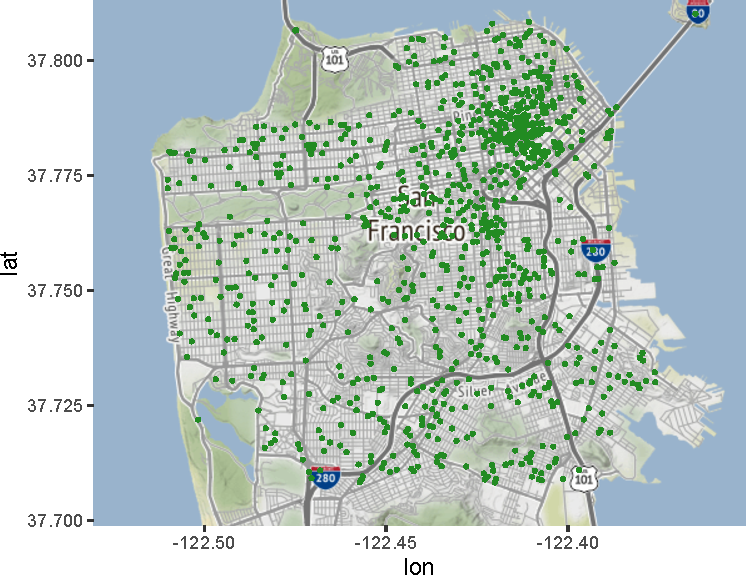
\includegraphics[width=1\linewidth,height=0.45\textheight,]{crimebythenumbers_files/figure-latex/unnamed-chunk-9-1}

When you run the above code it shows a world map (copied
several times). Zoom into it and it'll start showing
relevant features of wherever you're looking.

Note the \texttt{\%\textgreater{}\%} between the
\texttt{leaflet()} function and the \texttt{addTiles()}
function. \texttt{leaflet} is one of the packages in R where
we can use pipes.

To add the points to the graph we use the function
\texttt{addMarkers()} which has two parameters, \texttt{lng}
and \texttt{lat}. For both parameters we put the column in
which the longitude and latitude are, respectively.

\begin{Shaded}
\begin{Highlighting}[]
\FunctionTok{leaflet}\NormalTok{() }\SpecialCharTok{\%\textgreater{}\%}
  \FunctionTok{addTiles}\NormalTok{(}\StringTok{"http://\{s\}.tile.openstreetmap.org/\{z\}/\{x\}/\{y\}.png"}\NormalTok{,}
    \AttributeTok{attribution =} \StringTok{\textquotesingle{}\&copy; \textless{}a href="http://openstreetmap.org"\textgreater{}}
\StringTok{                OpenStreetMap\textless{}/a\textgreater{} contributors\textquotesingle{}}
\NormalTok{  ) }\SpecialCharTok{\%\textgreater{}\%}
  \FunctionTok{addMarkers}\NormalTok{(}
    \AttributeTok{lng =}\NormalTok{ marijuana}\SpecialCharTok{$}\NormalTok{long,}
    \AttributeTok{lat =}\NormalTok{ marijuana}\SpecialCharTok{$}\NormalTok{lat}
\NormalTok{  )}
\end{Highlighting}
\end{Shaded}

\textbackslash begin\{center\}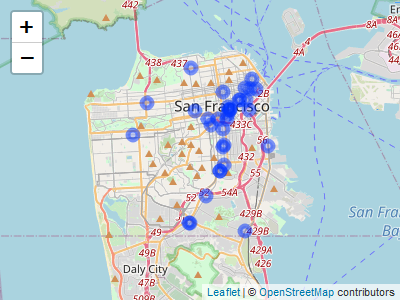
\includegraphics[width=1\linewidth,height=0.45\textheight,]{crimebythenumbers_files/figure-latex/unnamed-chunk-10-1}

It now adds an icon indicating where every dispensary in our
data is. You can zoom in and scroll around to see more about
where the dispensaries are. There are only a few dozen
locations in the data so the popups overlapping a bit
doesn't affect our map too much. If we had more - such as
crime data with millions of offenses - it would make it very
hard to read. To change the icons to circles we can change
the function \texttt{addMarkers()} to
\texttt{addCircleMarkers()}, keeping the rest of the code
the same.

\begin{Shaded}
\begin{Highlighting}[]
\FunctionTok{leaflet}\NormalTok{() }\SpecialCharTok{\%\textgreater{}\%}
  \FunctionTok{addTiles}\NormalTok{(}\StringTok{"http://\{s\}.tile.openstreetmap.org/\{z\}/\{x\}/\{y\}.png"}\NormalTok{,}
    \AttributeTok{attribution =} \StringTok{\textquotesingle{}\&copy; \textless{}a href="http://openstreetmap.org"\textgreater{}}
\StringTok{                OpenStreetMap\textless{}/a\textgreater{} contributors\textquotesingle{}}
\NormalTok{  ) }\SpecialCharTok{\%\textgreater{}\%}
  \FunctionTok{addCircleMarkers}\NormalTok{(}
    \AttributeTok{lng =}\NormalTok{ marijuana}\SpecialCharTok{$}\NormalTok{long,}
    \AttributeTok{lat =}\NormalTok{ marijuana}\SpecialCharTok{$}\NormalTok{lat}
\NormalTok{  )}
\end{Highlighting}
\end{Shaded}

\textbackslash begin\{center\}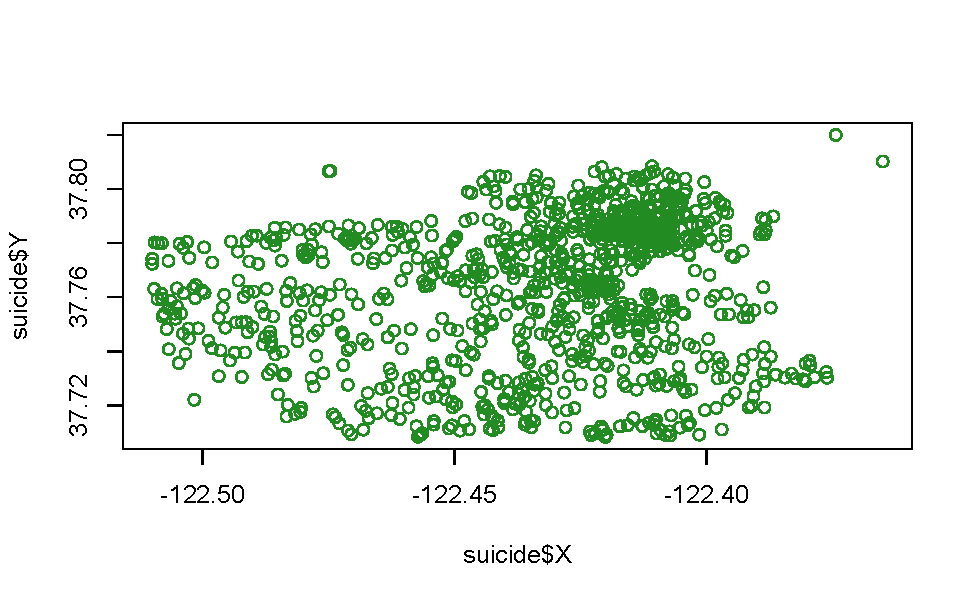
\includegraphics[width=1\linewidth,height=0.45\textheight,]{crimebythenumbers_files/figure-latex/unnamed-chunk-11-1}

This makes the icon into circles which take up less space
than icons. To adjust the size of our icons we use the
\texttt{radius} parameter in \texttt{addMarkers()} or
\texttt{addCircleMarkers()}. The larger the radius, the
larger the icons.

\begin{Shaded}
\begin{Highlighting}[]
\FunctionTok{leaflet}\NormalTok{() }\SpecialCharTok{\%\textgreater{}\%}
  \FunctionTok{addTiles}\NormalTok{(}\StringTok{"http://\{s\}.tile.openstreetmap.org/\{z\}/\{x\}/\{y\}.png"}\NormalTok{,}
    \AttributeTok{attribution =} \StringTok{\textquotesingle{}\&copy; \textless{}a href="http://openstreetmap.org"\textgreater{}}
\StringTok{                OpenStreetMap\textless{}/a\textgreater{} contributors\textquotesingle{}}
\NormalTok{  ) }\SpecialCharTok{\%\textgreater{}\%}
  \FunctionTok{addCircleMarkers}\NormalTok{(}
    \AttributeTok{lng =}\NormalTok{ marijuana}\SpecialCharTok{$}\NormalTok{long,}
    \AttributeTok{lat =}\NormalTok{ marijuana}\SpecialCharTok{$}\NormalTok{lat,}
    \AttributeTok{radius =} \DecValTok{5}
\NormalTok{  )}
\end{Highlighting}
\end{Shaded}

\textbackslash begin\{center\}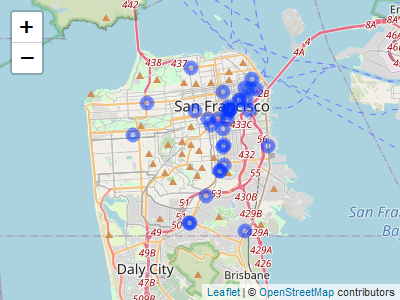
\includegraphics[width=1\linewidth,height=0.45\textheight,]{crimebythenumbers_files/figure-latex/unnamed-chunk-12-1}

Setting the \texttt{radius} option to 5 shrinks the size of
the icon a lot. In your own maps you'll have to fiddle with
this option to get it to look the way you want. Let's move
on to adding information about each icon when clicked upon.

\hypertarget{adding-popup-information}{%
\section{Adding popup
information}\label{adding-popup-information}}

The parameter \texttt{popup} in the \texttt{addMarkers()} or
\texttt{addCircleMarkers()} functions lets you input a
character value (if not already a character value it will
convert it to one) and that will be shown as a popup when
you click on the icon. Let's start simple here by inputting
the business owner column in our data and then build it up
to a more complicated popup.

\begin{Shaded}
\begin{Highlighting}[]
\FunctionTok{leaflet}\NormalTok{() }\SpecialCharTok{\%\textgreater{}\%}
  \FunctionTok{addTiles}\NormalTok{(}\StringTok{"http://\{s\}.tile.openstreetmap.org/\{z\}/\{x\}/\{y\}.png"}\NormalTok{,}
    \AttributeTok{attribution =} \StringTok{\textquotesingle{}\&copy; \textless{}a href="http://openstreetmap.org"\textgreater{}}
\StringTok{                OpenStreetMap\textless{}/a\textgreater{} contributors\textquotesingle{}}
\NormalTok{  ) }\SpecialCharTok{\%\textgreater{}\%}
  \FunctionTok{addCircleMarkers}\NormalTok{(}
    \AttributeTok{lng =}\NormalTok{ marijuana}\SpecialCharTok{$}\NormalTok{long,}
    \AttributeTok{lat =}\NormalTok{ marijuana}\SpecialCharTok{$}\NormalTok{lat,}
    \AttributeTok{radius =} \DecValTok{5}\NormalTok{,}
    \AttributeTok{popup =}\NormalTok{ marijuana}\SpecialCharTok{$}\NormalTok{Business\_Owner}
\NormalTok{  )}
\end{Highlighting}
\end{Shaded}

\textbackslash begin\{center\}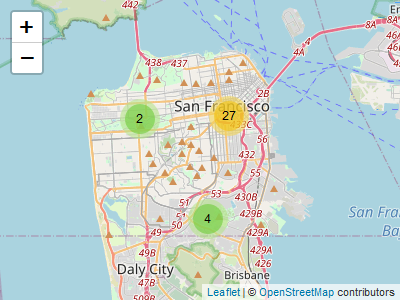
\includegraphics[width=1\linewidth,height=0.45\textheight,]{crimebythenumbers_files/figure-latex/unnamed-chunk-13-1}

Try clicking around and you'll see that the owner of the
dispensary you clicked on appears over the dot. We usually
want to have a title indicating what the value in the popup
means. We can do this by using the \texttt{paste()} function
to combine text explaining the value with the value itself.
Let's add the words ``Business Owner:'' before the business
owner column.

\begin{Shaded}
\begin{Highlighting}[]
\FunctionTok{leaflet}\NormalTok{() }\SpecialCharTok{\%\textgreater{}\%}
  \FunctionTok{addTiles}\NormalTok{(}\StringTok{"http://\{s\}.tile.openstreetmap.org/\{z\}/\{x\}/\{y\}.png"}\NormalTok{,}
    \AttributeTok{attribution =} \StringTok{\textquotesingle{}\&copy; \textless{}a href="http://openstreetmap.org"\textgreater{}}
\StringTok{                OpenStreetMap\textless{}/a\textgreater{} contributors\textquotesingle{}}
\NormalTok{  ) }\SpecialCharTok{\%\textgreater{}\%}
  \FunctionTok{addCircleMarkers}\NormalTok{(}
    \AttributeTok{lng =}\NormalTok{ marijuana}\SpecialCharTok{$}\NormalTok{long,}
    \AttributeTok{lat =}\NormalTok{ marijuana}\SpecialCharTok{$}\NormalTok{lat,}
    \AttributeTok{radius =} \DecValTok{5}\NormalTok{,}
    \AttributeTok{popup =} \FunctionTok{paste}\NormalTok{(}
      \StringTok{"Business Owner:"}\NormalTok{,}
\NormalTok{      marijuana}\SpecialCharTok{$}\NormalTok{Business\_Owner}
\NormalTok{    )}
\NormalTok{  )}
\end{Highlighting}
\end{Shaded}

\textbackslash begin\{center\}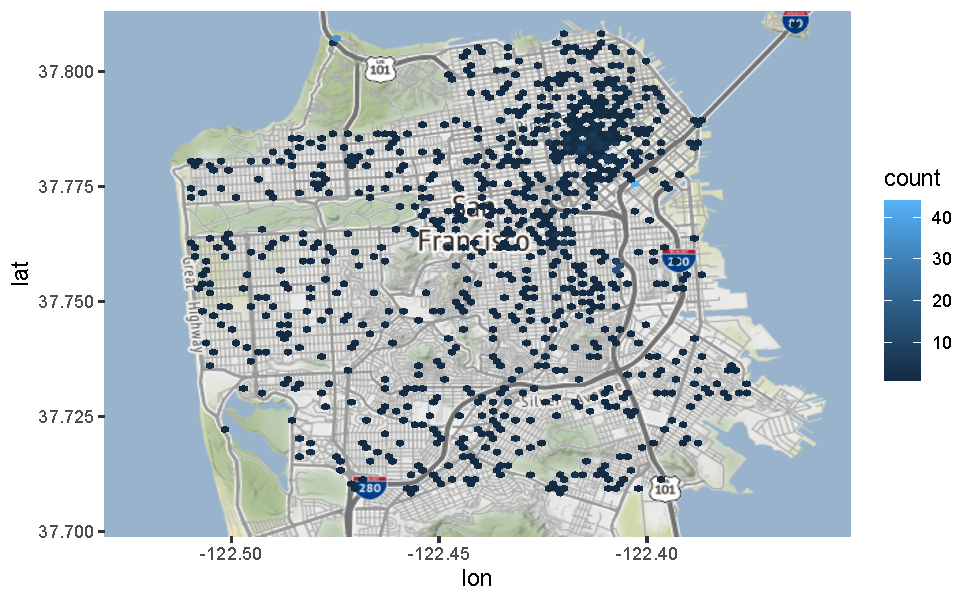
\includegraphics[width=1\linewidth,height=0.45\textheight,]{crimebythenumbers_files/figure-latex/unnamed-chunk-14-1}

We don't have too much information in the data but we let's
add the address and license number to the popup by adding
them to the \texttt{paste()} function we're using.

\begin{Shaded}
\begin{Highlighting}[]
\FunctionTok{leaflet}\NormalTok{() }\SpecialCharTok{\%\textgreater{}\%}
  \FunctionTok{addTiles}\NormalTok{(}\StringTok{"http://\{s\}.tile.openstreetmap.org/\{z\}/\{x\}/\{y\}.png"}\NormalTok{,}
    \AttributeTok{attribution =} \StringTok{\textquotesingle{}\&copy; \textless{}a href="http://openstreetmap.org"\textgreater{}}
\StringTok{                OpenStreetMap\textless{}/a\textgreater{} contributors\textquotesingle{}}
\NormalTok{  ) }\SpecialCharTok{\%\textgreater{}\%}
  \FunctionTok{addCircleMarkers}\NormalTok{(}
    \AttributeTok{lng =}\NormalTok{ marijuana}\SpecialCharTok{$}\NormalTok{long,}
    \AttributeTok{lat =}\NormalTok{ marijuana}\SpecialCharTok{$}\NormalTok{lat,}
    \AttributeTok{radius =} \DecValTok{5}\NormalTok{,}
    \AttributeTok{popup =} \FunctionTok{paste}\NormalTok{(}
      \StringTok{"Business Owner:"}\NormalTok{,}
\NormalTok{      marijuana}\SpecialCharTok{$}\NormalTok{Business\_Owner,}
      \StringTok{"Address:"}\NormalTok{,}
\NormalTok{      marijuana}\SpecialCharTok{$}\NormalTok{Premise\_Address,}
      \StringTok{"License:"}\NormalTok{,}
\NormalTok{      marijuana}\SpecialCharTok{$}\NormalTok{License\_Number}
\NormalTok{    )}
\NormalTok{  )}
\end{Highlighting}
\end{Shaded}

\textbackslash begin\{center\}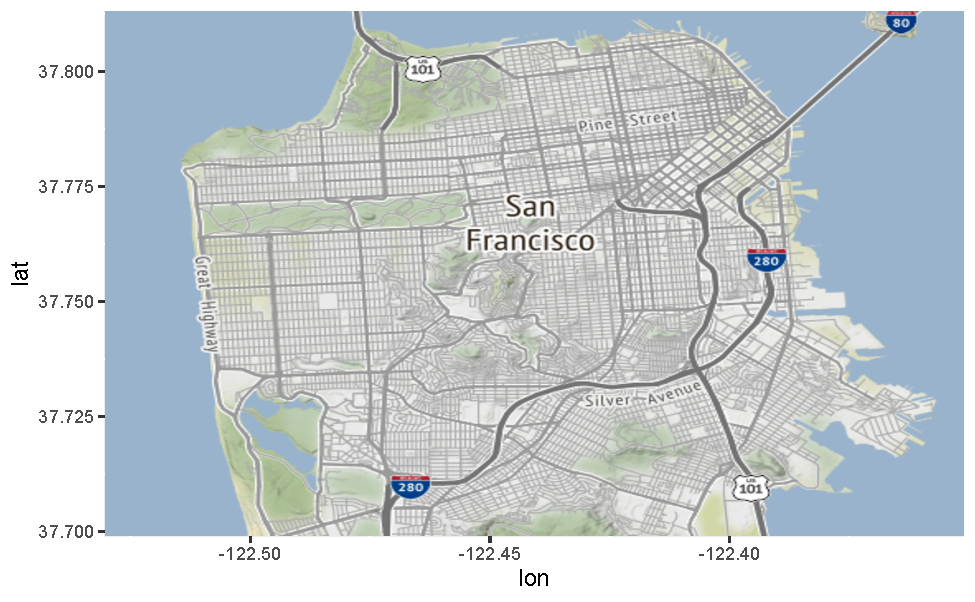
\includegraphics[width=1\linewidth,height=0.45\textheight,]{crimebythenumbers_files/figure-latex/unnamed-chunk-15-1}

Just adding the location text makes it try to print out
everything on one line which is hard to read. If we add the
text \texttt{\textless{}br\textgreater{}} where we want a
line break it will make one.
\texttt{\textless{}br\textgreater{}} is the HTML tag for
line-break which is why it works making a new line in this
case.

\begin{Shaded}
\begin{Highlighting}[]
\FunctionTok{leaflet}\NormalTok{() }\SpecialCharTok{\%\textgreater{}\%}
  \FunctionTok{addTiles}\NormalTok{(}\StringTok{"http://\{s\}.tile.openstreetmap.org/\{z\}/\{x\}/\{y\}.png"}\NormalTok{,}
    \AttributeTok{attribution =} \StringTok{\textquotesingle{}\&copy; \textless{}a href="http://openstreetmap.org"\textgreater{}}
\StringTok{                OpenStreetMap\textless{}/a\textgreater{} contributors\textquotesingle{}}
\NormalTok{  ) }\SpecialCharTok{\%\textgreater{}\%}
  \FunctionTok{addCircleMarkers}\NormalTok{(}
    \AttributeTok{lng =}\NormalTok{ marijuana}\SpecialCharTok{$}\NormalTok{long,}
    \AttributeTok{lat =}\NormalTok{ marijuana}\SpecialCharTok{$}\NormalTok{lat,}
    \AttributeTok{radius =} \DecValTok{5}\NormalTok{,}
    \AttributeTok{popup =} \FunctionTok{paste}\NormalTok{(}
      \StringTok{"Business Owner:"}\NormalTok{,}
\NormalTok{      marijuana}\SpecialCharTok{$}\NormalTok{Business\_Owner,}
      \StringTok{"\textless{}br\textgreater{}"}\NormalTok{,}
      \StringTok{"Address:"}\NormalTok{,}
\NormalTok{      marijuana}\SpecialCharTok{$}\NormalTok{Premise\_Address,}
      \StringTok{"\textless{}br\textgreater{}"}\NormalTok{,}
      \StringTok{"License:"}\NormalTok{,}
\NormalTok{      marijuana}\SpecialCharTok{$}\NormalTok{License\_Number}
\NormalTok{    )}
\NormalTok{  )}
\end{Highlighting}
\end{Shaded}

\textbackslash begin\{center\}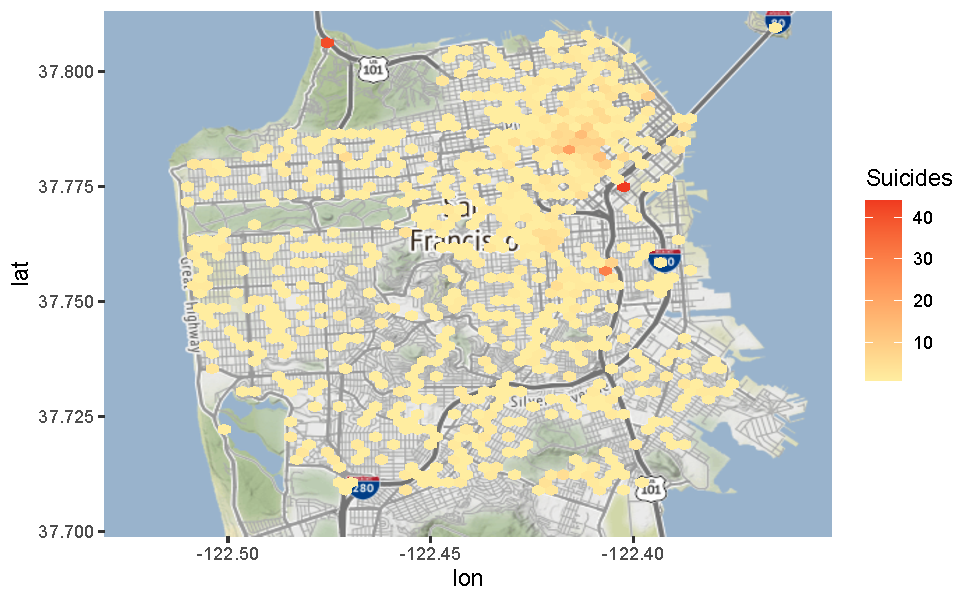
\includegraphics[width=1\linewidth,height=0.45\textheight,]{crimebythenumbers_files/figure-latex/unnamed-chunk-16-1}

\hypertarget{dealing-with-too-many-markers}{%
\section{Dealing with too many
markers}\label{dealing-with-too-many-markers}}

In our case with only 33 rows of data, turning the markers
to circles solves our visibility issue. In cases with many
more rows of data, this doesn't always work. A solution for
this is to cluster the data into groups where the dots only
show if you zoom in.

If we add the code
\texttt{clusterOptions\ =\ markerClusterOptions()} to our
\texttt{addCircleMarkers()} it will cluster for us.

\begin{Shaded}
\begin{Highlighting}[]
\FunctionTok{leaflet}\NormalTok{() }\SpecialCharTok{\%\textgreater{}\%}
  \FunctionTok{addTiles}\NormalTok{(}\StringTok{"http://\{s\}.tile.openstreetmap.org/\{z\}/\{x\}/\{y\}.png"}\NormalTok{,}
    \AttributeTok{attribution =} \StringTok{\textquotesingle{}\&copy; \textless{}a href="http://openstreetmap.org"\textgreater{}}
\StringTok{                OpenStreetMap\textless{}/a\textgreater{} contributors\textquotesingle{}}
\NormalTok{  ) }\SpecialCharTok{\%\textgreater{}\%}
  \FunctionTok{addCircleMarkers}\NormalTok{(}
    \AttributeTok{lng =}\NormalTok{ marijuana}\SpecialCharTok{$}\NormalTok{long,}
    \AttributeTok{lat =}\NormalTok{ marijuana}\SpecialCharTok{$}\NormalTok{lat,}
    \AttributeTok{radius =} \DecValTok{5}\NormalTok{,}
    \AttributeTok{popup =} \FunctionTok{paste}\NormalTok{(}
      \StringTok{"Business Owner:"}\NormalTok{,}
\NormalTok{      marijuana}\SpecialCharTok{$}\NormalTok{Business\_Owner,}
      \StringTok{"\textless{}br\textgreater{}"}\NormalTok{,}
      \StringTok{"Address:"}\NormalTok{,}
\NormalTok{      marijuana}\SpecialCharTok{$}\NormalTok{Premise\_Address,}
      \StringTok{"\textless{}br\textgreater{}"}\NormalTok{,}
      \StringTok{"License:"}\NormalTok{,}
\NormalTok{      marijuana}\SpecialCharTok{$}\NormalTok{License\_Number}
\NormalTok{    ),}
    \AttributeTok{clusterOptions =} \FunctionTok{markerClusterOptions}\NormalTok{()}
\NormalTok{  )}
\end{Highlighting}
\end{Shaded}

\textbackslash begin\{center\}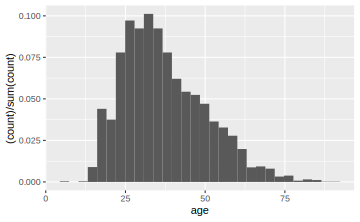
\includegraphics[width=1\linewidth,height=0.45\textheight,]{crimebythenumbers_files/figure-latex/unnamed-chunk-17-1}

Locations close to each other are grouped together in fairly
arbitrary groupings and we can see how large each grouping
is by moving our cursor over the circle. Click on a circle
or zoom in and it will show smaller groupings at lower
levels of aggregation. Keep clicking or zooming in and it
will eventually show each location as its own circle.

This method is very useful for dealing with huge amounts of
data as it avoids overflowing the map with too many icons at
one time. A downside, however, is that the clusters are
created arbitrarily meaning that important context, such as
neighborhood, can be lost.

\hypertarget{interactive-choropleth-maps}{%
\section{Interactive choropleth
maps}\label{interactive-choropleth-maps}}

In Chapter @ref(choropleth-maps) we worked on choropleth
maps which are maps with shaded regions, such as states
colored by which political party won them in an election.
Here we will make interactive choropleth maps where you can
click on a shaded region and see information about that
region. We'll make the same map as before - neighborhoods
shaded by the number of suicides.

Let's load the San Francisco suicides-by-neighborhood data
that we made earlier. We'll also want to project it to the
standard longitude and latitude projection.

\begin{Shaded}
\begin{Highlighting}[]
\FunctionTok{library}\NormalTok{(sf)}
\FunctionTok{load}\NormalTok{(}\StringTok{"data/sf\_neighborhoods\_suicide.rda"}\NormalTok{)}
\NormalTok{sf\_neighborhoods\_suicide }\OtherTok{\textless{}{-}} \FunctionTok{st\_transform}\NormalTok{(}
\NormalTok{  sf\_neighborhoods\_suicide,}
  \StringTok{"+proj=longlat +datum=WGS84"}
\NormalTok{)}
\end{Highlighting}
\end{Shaded}

We'll begin the \texttt{leaflet} map similar to before but
use the function \texttt{addPolygons()} and our input here
is the geometry column of \emph{sf\_neighborhoods\_suicide}.

\begin{Shaded}
\begin{Highlighting}[]
\FunctionTok{leaflet}\NormalTok{() }\SpecialCharTok{\%\textgreater{}\%}
  \FunctionTok{addTiles}\NormalTok{(}\StringTok{"http://\{s\}.tile.openstreetmap.org/\{z\}/\{x\}/\{y\}.png"}\NormalTok{,}
    \AttributeTok{attribution =} \StringTok{\textquotesingle{}\&copy; \textless{}a href="http://openstreetmap.org"\textgreater{}}
\StringTok{                OpenStreetMap\textless{}/a\textgreater{} contributors\textquotesingle{}}
\NormalTok{  ) }\SpecialCharTok{\%\textgreater{}\%}
  \FunctionTok{addPolygons}\NormalTok{(}\AttributeTok{data =}\NormalTok{ sf\_neighborhoods\_suicide}\SpecialCharTok{$}\NormalTok{geometry)}
\end{Highlighting}
\end{Shaded}

\textbackslash begin\{center\}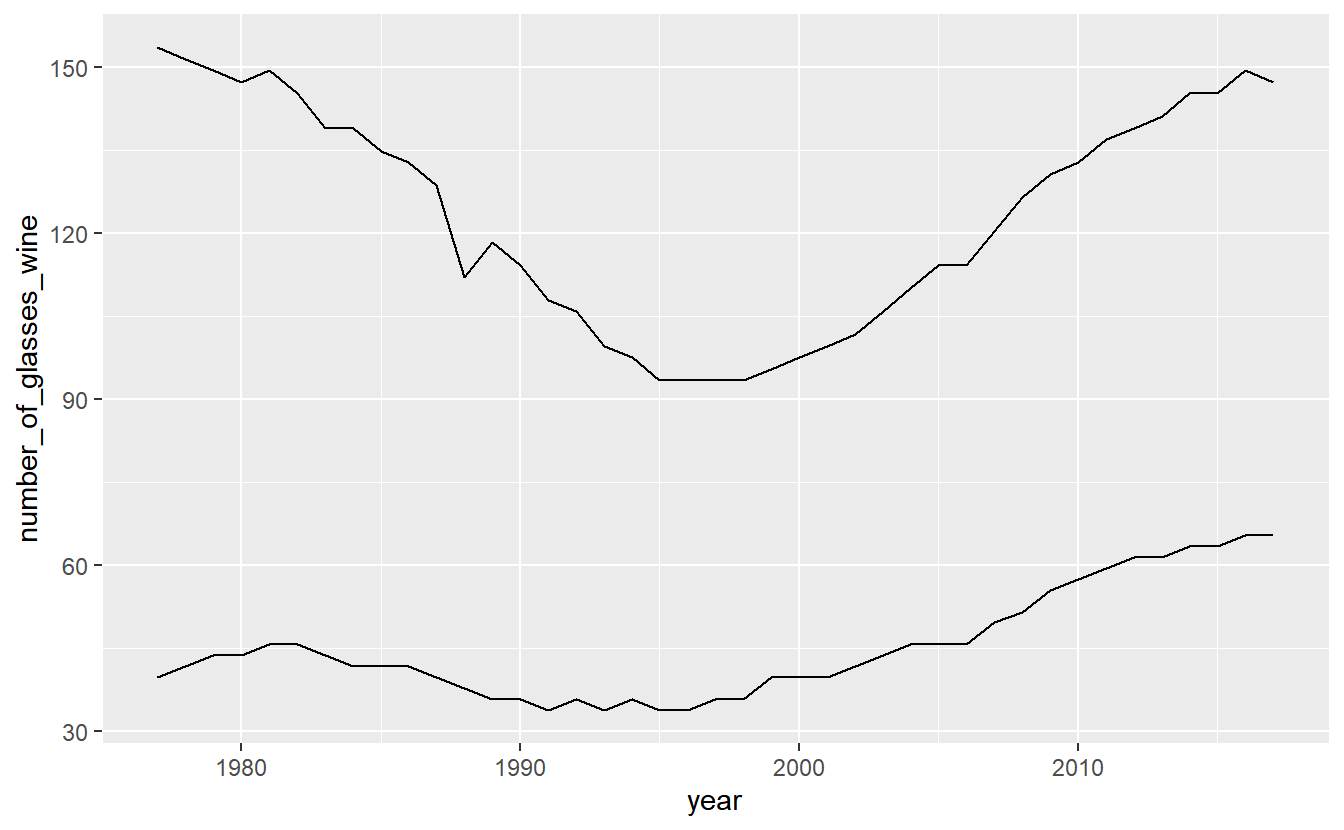
\includegraphics[width=1\linewidth,height=0.45\textheight,]{crimebythenumbers_files/figure-latex/unnamed-chunk-19-1}

It gives us a blank map because our polygons are projected
to San Francisco's projection while the \texttt{leaflet} map
expects the standard CRS, WGS84 which uses longitude and
latitude. So we need to change our projection to that using
the \texttt{st\_transform()} function from the \texttt{sf}
package.

\begin{Shaded}
\begin{Highlighting}[]
\FunctionTok{library}\NormalTok{(sf)}
\NormalTok{sf\_neighborhoods\_suicide }\OtherTok{\textless{}{-}} \FunctionTok{st\_transform}\NormalTok{(sf\_neighborhoods\_suicide,}
  \AttributeTok{crs =} \StringTok{"+proj=longlat +datum=WGS84"}
\NormalTok{)}
\end{Highlighting}
\end{Shaded}

Now let's try again.

\begin{Shaded}
\begin{Highlighting}[]
\FunctionTok{leaflet}\NormalTok{() }\SpecialCharTok{\%\textgreater{}\%}
  \FunctionTok{addTiles}\NormalTok{(}\StringTok{"http://\{s\}.tile.openstreetmap.org/\{z\}/\{x\}/\{y\}.png"}\NormalTok{,}
    \AttributeTok{attribution =} \StringTok{\textquotesingle{}\&copy; \textless{}a href="http://openstreetmap.org"\textgreater{}}
\StringTok{                OpenStreetMap\textless{}/a\textgreater{} contributors\textquotesingle{}}
\NormalTok{  ) }\SpecialCharTok{\%\textgreater{}\%}
  \FunctionTok{addPolygons}\NormalTok{(}\AttributeTok{data =}\NormalTok{ sf\_neighborhoods\_suicide}\SpecialCharTok{$}\NormalTok{geometry)}
\end{Highlighting}
\end{Shaded}

\textbackslash begin\{center\}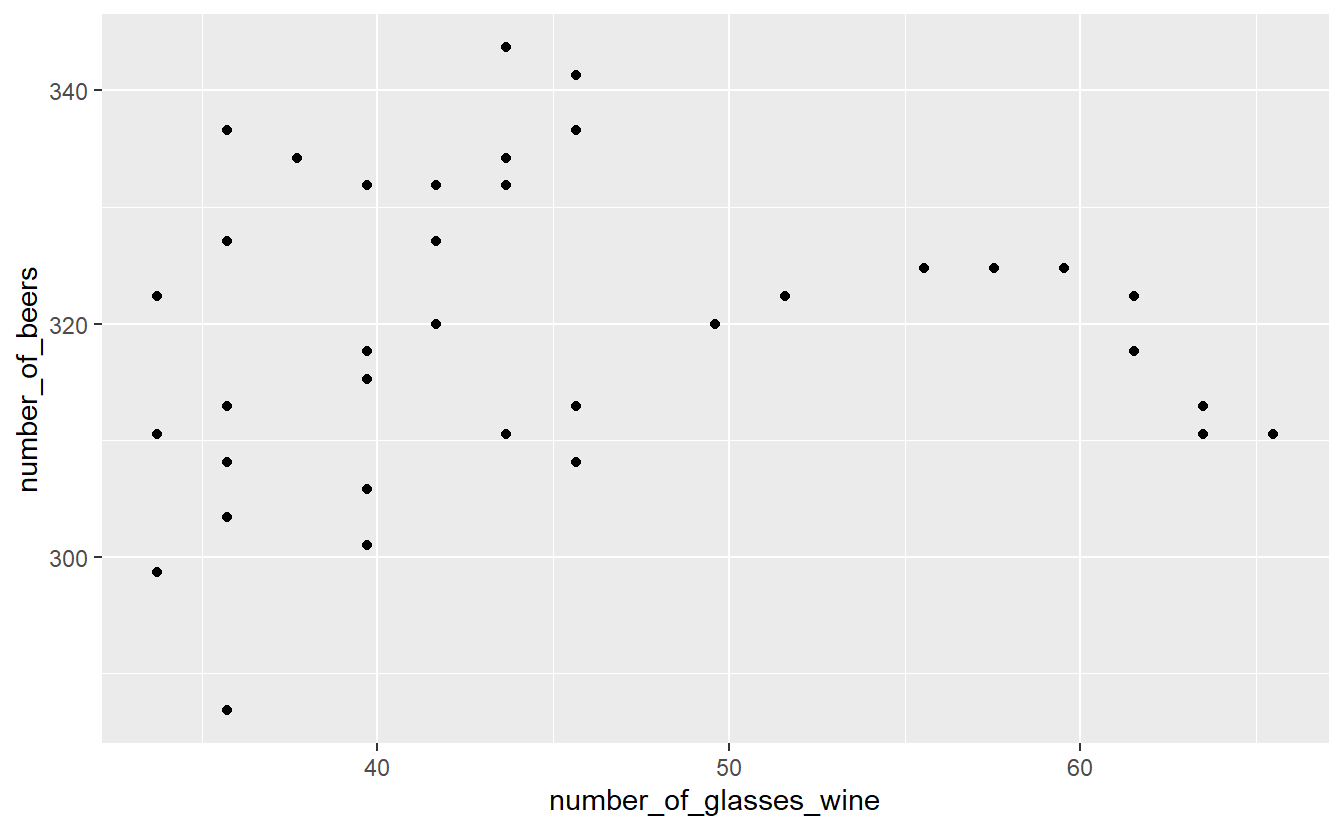
\includegraphics[width=1\linewidth,height=0.45\textheight,]{crimebythenumbers_files/figure-latex/unnamed-chunk-21-1}

It made a map with thick blue lines indicating each
neighborhood. Let's change the appearance of the graph a bit
before making a popup or shading the neighborhoods The
parameter \texttt{color} in \texttt{addPolygons()} changes
the color of the lines - let's change it to black. The lines
are also very thick, blurring into each other and making the
neighborhoods hard to see. We can change the \texttt{weight}
parameter to alter the size of these lines - smaller values
are thinner lines. Let's try setting this to 1.

\begin{Shaded}
\begin{Highlighting}[]
\FunctionTok{leaflet}\NormalTok{() }\SpecialCharTok{\%\textgreater{}\%}
  \FunctionTok{addTiles}\NormalTok{(}\StringTok{"http://\{s\}.tile.openstreetmap.org/\{z\}/\{x\}/\{y\}.png"}\NormalTok{,}
    \AttributeTok{attribution =} \StringTok{\textquotesingle{}\&copy; \textless{}a href="http://openstreetmap.org"\textgreater{}}
\StringTok{                OpenStreetMap\textless{}/a\textgreater{} contributors\textquotesingle{}}
\NormalTok{  ) }\SpecialCharTok{\%\textgreater{}\%}
  \FunctionTok{addPolygons}\NormalTok{(}
    \AttributeTok{data =}\NormalTok{ sf\_neighborhoods\_suicide}\SpecialCharTok{$}\NormalTok{geometry,}
    \AttributeTok{color =} \StringTok{"black"}\NormalTok{,}
    \AttributeTok{weight =} \DecValTok{1}
\NormalTok{  )}
\end{Highlighting}
\end{Shaded}

\textbackslash begin\{center\}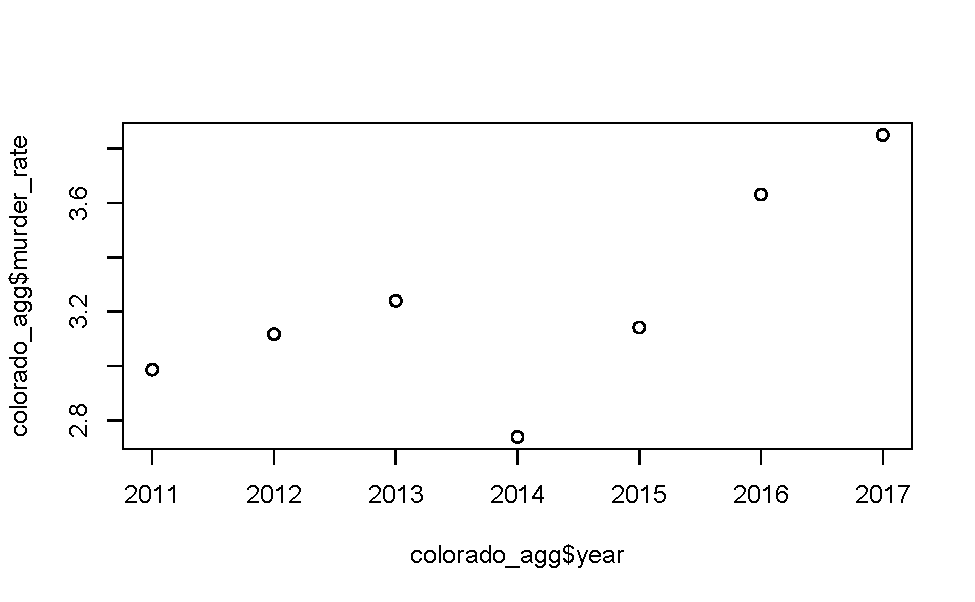
\includegraphics[width=1\linewidth,height=0.45\textheight,]{crimebythenumbers_files/figure-latex/unnamed-chunk-22-1}

That looks better and we can clearly distinguish each
neighborhood now.

As we did earlier, we can add the popup text directly to the
function which makes the geographic shapes, in this case
\texttt{addPolygons()}. Let's add the \emph{nhood} column
value - the name of that neighborhood - and the number of
suicides that occurred in that neighborhood. As before, when
we click on a neighborhood a popup appears with the output
we specified.

\begin{Shaded}
\begin{Highlighting}[]
\FunctionTok{leaflet}\NormalTok{() }\SpecialCharTok{\%\textgreater{}\%}
  \FunctionTok{addTiles}\NormalTok{(}\StringTok{"http://\{s\}.tile.openstreetmap.org/\{z\}/\{x\}/\{y\}.png"}\NormalTok{,}
    \AttributeTok{attribution =} \StringTok{\textquotesingle{}\&copy; \textless{}a href="http://openstreetmap.org"\textgreater{}}
\StringTok{                OpenStreetMap\textless{}/a\textgreater{} contributors\textquotesingle{}}
\NormalTok{  ) }\SpecialCharTok{\%\textgreater{}\%}
  \FunctionTok{addPolygons}\NormalTok{(}
    \AttributeTok{data =}\NormalTok{ sf\_neighborhoods\_suicide}\SpecialCharTok{$}\NormalTok{geometry,}
    \AttributeTok{col =} \StringTok{"black"}\NormalTok{,}
    \AttributeTok{weight =} \DecValTok{1}\NormalTok{,}
    \AttributeTok{popup =} \FunctionTok{paste0}\NormalTok{(}
      \StringTok{"Neighborhood: "}\NormalTok{,}
\NormalTok{      sf\_neighborhoods\_suicide}\SpecialCharTok{$}\NormalTok{nhood,}
      \StringTok{"\textless{}br\textgreater{}"}\NormalTok{,}
      \StringTok{"Number of Suicides: "}\NormalTok{,}
\NormalTok{      sf\_neighborhoods\_suicide}\SpecialCharTok{$}\NormalTok{number\_suicides}
\NormalTok{    )}
\NormalTok{  )}
\end{Highlighting}
\end{Shaded}

\textbackslash begin\{center\}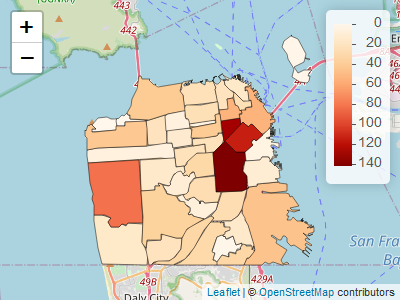
\includegraphics[width=1\linewidth,height=0.45\textheight,]{crimebythenumbers_files/figure-latex/unnamed-chunk-23-1}

For these types of maps we generally want to shade each
polygon to indicate how frequently the event occurred in the
polygon. We'll use the function \texttt{colorNumeric()}
which takes a lot of the work out of the process of coloring
in the map. This function takes two inputs, first a color
palette which we can get from the site
\href{http://colorbrewer2.org/\#type=sequential\&scheme=OrRd\&n=3}{Color
Brewer}. Let's use the fourth bar in the Sequential page,
which is light orange to red. If you look in the section
with each HEX value it says that the palette is ``3-class
OrRd''. The ``3-class'' just means we selected 3 colors, the
``OrRd'' is the part we want. That will tell
\texttt{colorNumeric()} to make the palette using these
colors. The second parameter is the column for our numeric
variable, \emph{number\_suicides}.

We will save the output of
\texttt{colorNumeric("OrRd",\ sf\_neighborhoods\_suicide\$number\_suicides)}
as a new object which we'll call \emph{pal} for convenience
since it is a palette of colors. Then inside of
\texttt{addPolygons()} we'll set the parameter
\texttt{fillColor} to
\texttt{pal(sf\_neighborhoods\_suicide\$number\_suicides)},
running this function on the column. What this really does
is determine which color every neighborhood should be based
on the value in the \emph{number\_suicides} column.

\begin{Shaded}
\begin{Highlighting}[]
\NormalTok{pal }\OtherTok{\textless{}{-}} \FunctionTok{colorNumeric}\NormalTok{(}\StringTok{"OrRd"}\NormalTok{, sf\_neighborhoods\_suicide}\SpecialCharTok{$}\NormalTok{number\_suicides)}
\FunctionTok{leaflet}\NormalTok{() }\SpecialCharTok{\%\textgreater{}\%}
  \FunctionTok{addTiles}\NormalTok{(}\StringTok{"http://\{s\}.tile.openstreetmap.org/\{z\}/\{x\}/\{y\}.png"}\NormalTok{,}
    \AttributeTok{attribution =} \StringTok{\textquotesingle{}\&copy; \textless{}a href="http://openstreetmap.org"\textgreater{}}
\StringTok{                OpenStreetMap\textless{}/a\textgreater{} contributors\textquotesingle{}}
\NormalTok{  ) }\SpecialCharTok{\%\textgreater{}\%}
  \FunctionTok{addPolygons}\NormalTok{(}
    \AttributeTok{data =}\NormalTok{ sf\_neighborhoods\_suicide}\SpecialCharTok{$}\NormalTok{geometry,}
    \AttributeTok{col =} \StringTok{"black"}\NormalTok{,}
    \AttributeTok{weight =} \DecValTok{1}\NormalTok{,}
    \AttributeTok{popup =} \FunctionTok{paste0}\NormalTok{(}
      \StringTok{"Neighborhood: "}\NormalTok{,}
\NormalTok{      sf\_neighborhoods\_suicide}\SpecialCharTok{$}\NormalTok{nhood,}
      \StringTok{"\textless{}br\textgreater{}"}\NormalTok{,}
      \StringTok{"Number of Suicides: "}\NormalTok{,}
\NormalTok{      sf\_neighborhoods\_suicide}\SpecialCharTok{$}\NormalTok{number\_suicides}
\NormalTok{    ),}
    \AttributeTok{fillColor =} \FunctionTok{pal}\NormalTok{(sf\_neighborhoods\_suicide}\SpecialCharTok{$}\NormalTok{number\_suicides)}
\NormalTok{  )}
\end{Highlighting}
\end{Shaded}

\textbackslash begin\{center\}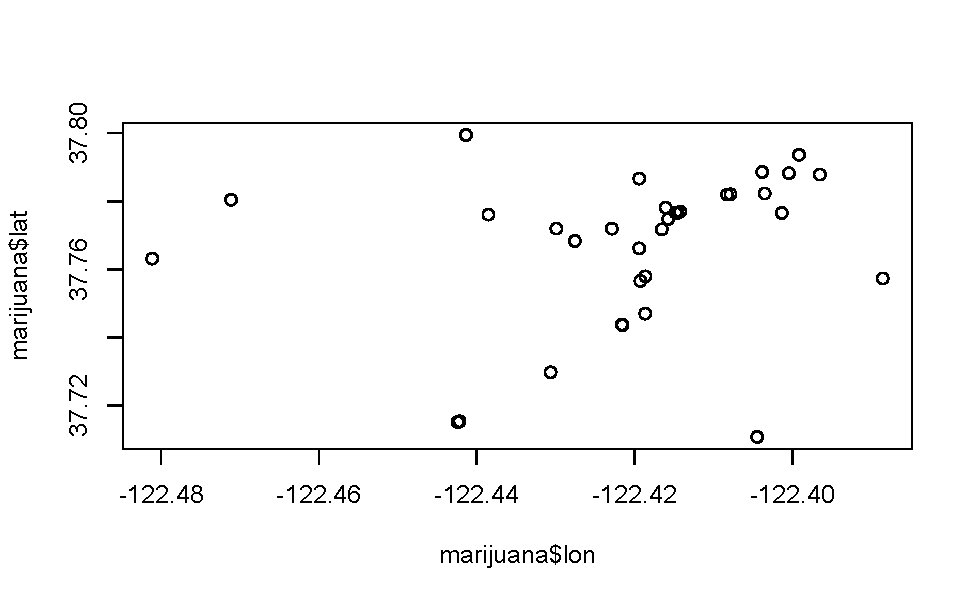
\includegraphics[width=1\linewidth,height=0.45\textheight,]{crimebythenumbers_files/figure-latex/unnamed-chunk-24-1}

Since the neighborhoods are transparent, it is hard to
distinguish which color is shown. We can make each
neighborhood a solid color by setting the parameter
\texttt{fillOpacity} inside of \texttt{addPolygons()} to 1.

\begin{Shaded}
\begin{Highlighting}[]
\NormalTok{pal }\OtherTok{\textless{}{-}} \FunctionTok{colorNumeric}\NormalTok{(}\StringTok{"OrRd"}\NormalTok{, sf\_neighborhoods\_suicide}\SpecialCharTok{$}\NormalTok{number\_suicides)}
\FunctionTok{leaflet}\NormalTok{() }\SpecialCharTok{\%\textgreater{}\%}
  \FunctionTok{addTiles}\NormalTok{(}\StringTok{"http://\{s\}.tile.openstreetmap.org/\{z\}/\{x\}/\{y\}.png"}\NormalTok{,}
    \AttributeTok{attribution =} \StringTok{\textquotesingle{}\&copy; \textless{}a href="http://openstreetmap.org"\textgreater{}}
\StringTok{                OpenStreetMap\textless{}/a\textgreater{} contributors\textquotesingle{}}
\NormalTok{  ) }\SpecialCharTok{\%\textgreater{}\%}
  \FunctionTok{addPolygons}\NormalTok{(}
    \AttributeTok{data =}\NormalTok{ sf\_neighborhoods\_suicide}\SpecialCharTok{$}\NormalTok{geometry,}
    \AttributeTok{col =} \StringTok{"black"}\NormalTok{,}
    \AttributeTok{weight =} \DecValTok{1}\NormalTok{,}
    \AttributeTok{popup =} \FunctionTok{paste0}\NormalTok{(}
      \StringTok{"Neighborhood: "}\NormalTok{,}
\NormalTok{      sf\_neighborhoods\_suicide}\SpecialCharTok{$}\NormalTok{nhood,}
      \StringTok{"\textless{}br\textgreater{}"}\NormalTok{,}
      \StringTok{"Number of Suicides: "}\NormalTok{,}
\NormalTok{      sf\_neighborhoods\_suicide}\SpecialCharTok{$}\NormalTok{number\_suicides}
\NormalTok{    ),}
    \AttributeTok{fillColor =} \FunctionTok{pal}\NormalTok{(sf\_neighborhoods\_suicide}\SpecialCharTok{$}\NormalTok{number\_suicides),}
    \AttributeTok{fillOpacity =} \DecValTok{1}
\NormalTok{  )}
\end{Highlighting}
\end{Shaded}

\textbackslash begin\{center\}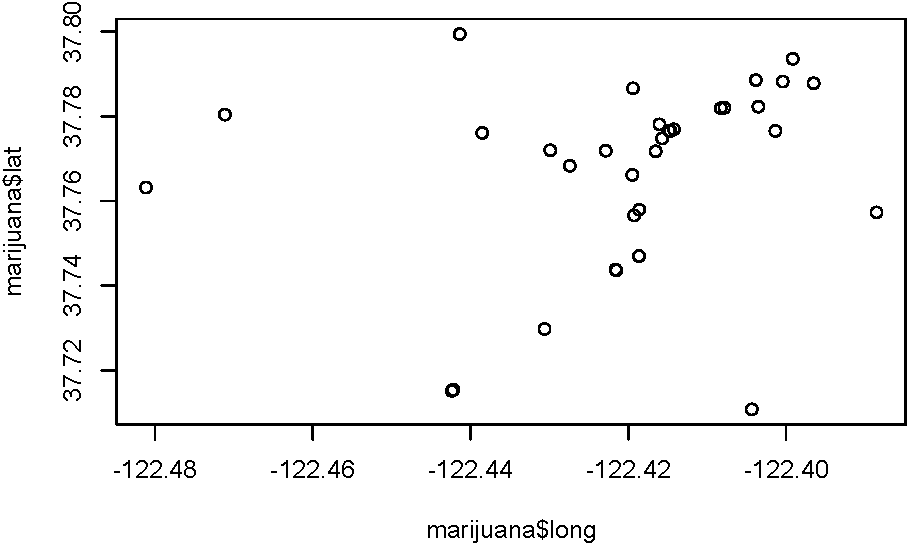
\includegraphics[width=1\linewidth,height=0.45\textheight,]{crimebythenumbers_files/figure-latex/unnamed-chunk-25-1}

To add a legend to this we use the function
\texttt{addLegend()} which takes three parameters.
\texttt{pal} asks which color palette we are using - we want
it to be the exact same as we use to color the neighborhoods
so we'll use the \emph{pal} object we made. The
\texttt{values} parameter is used for which column our
numeric values are from, in our case the
\emph{number\_suicides} column so we'll input that. Finally
\texttt{opacity} determines how transparent the legend will
be. As each neighborhood is set to not be transparent at
all, we'll also set this to 1 to be consistent.

\begin{Shaded}
\begin{Highlighting}[]
\NormalTok{pal }\OtherTok{\textless{}{-}} \FunctionTok{colorNumeric}\NormalTok{(}\StringTok{"OrRd"}\NormalTok{, sf\_neighborhoods\_suicide}\SpecialCharTok{$}\NormalTok{number\_suicides)}
\FunctionTok{leaflet}\NormalTok{() }\SpecialCharTok{\%\textgreater{}\%}
  \FunctionTok{addTiles}\NormalTok{(}\StringTok{"http://\{s\}.tile.openstreetmap.org/\{z\}/\{x\}/\{y\}.png"}\NormalTok{,}
    \AttributeTok{attribution =} \StringTok{\textquotesingle{}\&copy; \textless{}a href="http://openstreetmap.org"\textgreater{}}
\StringTok{                OpenStreetMap\textless{}/a\textgreater{} contributors\textquotesingle{}}
\NormalTok{  ) }\SpecialCharTok{\%\textgreater{}\%}
  \FunctionTok{addPolygons}\NormalTok{(}
    \AttributeTok{data =}\NormalTok{ sf\_neighborhoods\_suicide}\SpecialCharTok{$}\NormalTok{geometry,}
    \AttributeTok{col =} \StringTok{"black"}\NormalTok{,}
    \AttributeTok{weight =} \DecValTok{1}\NormalTok{,}
    \AttributeTok{popup =} \FunctionTok{paste0}\NormalTok{(}
      \StringTok{"Neighborhood: "}\NormalTok{,}
\NormalTok{      sf\_neighborhoods\_suicide}\SpecialCharTok{$}\NormalTok{nhood,}
      \StringTok{"\textless{}br\textgreater{}"}\NormalTok{,}
      \StringTok{"Number of Suicides: "}\NormalTok{,}
\NormalTok{      sf\_neighborhoods\_suicide}\SpecialCharTok{$}\NormalTok{number\_suicides}
\NormalTok{    ),}
    \AttributeTok{fillColor =} \FunctionTok{pal}\NormalTok{(sf\_neighborhoods\_suicide}\SpecialCharTok{$}\NormalTok{number\_suicides),}
    \AttributeTok{fillOpacity =} \DecValTok{1}
\NormalTok{  ) }\SpecialCharTok{\%\textgreater{}\%}
  \FunctionTok{addLegend}\NormalTok{(}
    \AttributeTok{pal =}\NormalTok{ pal,}
    \AttributeTok{values =}\NormalTok{ sf\_neighborhoods\_suicide}\SpecialCharTok{$}\NormalTok{number\_suicides,}
    \AttributeTok{opacity =} \DecValTok{1}
\NormalTok{  )}
\end{Highlighting}
\end{Shaded}

\textbackslash begin\{center\}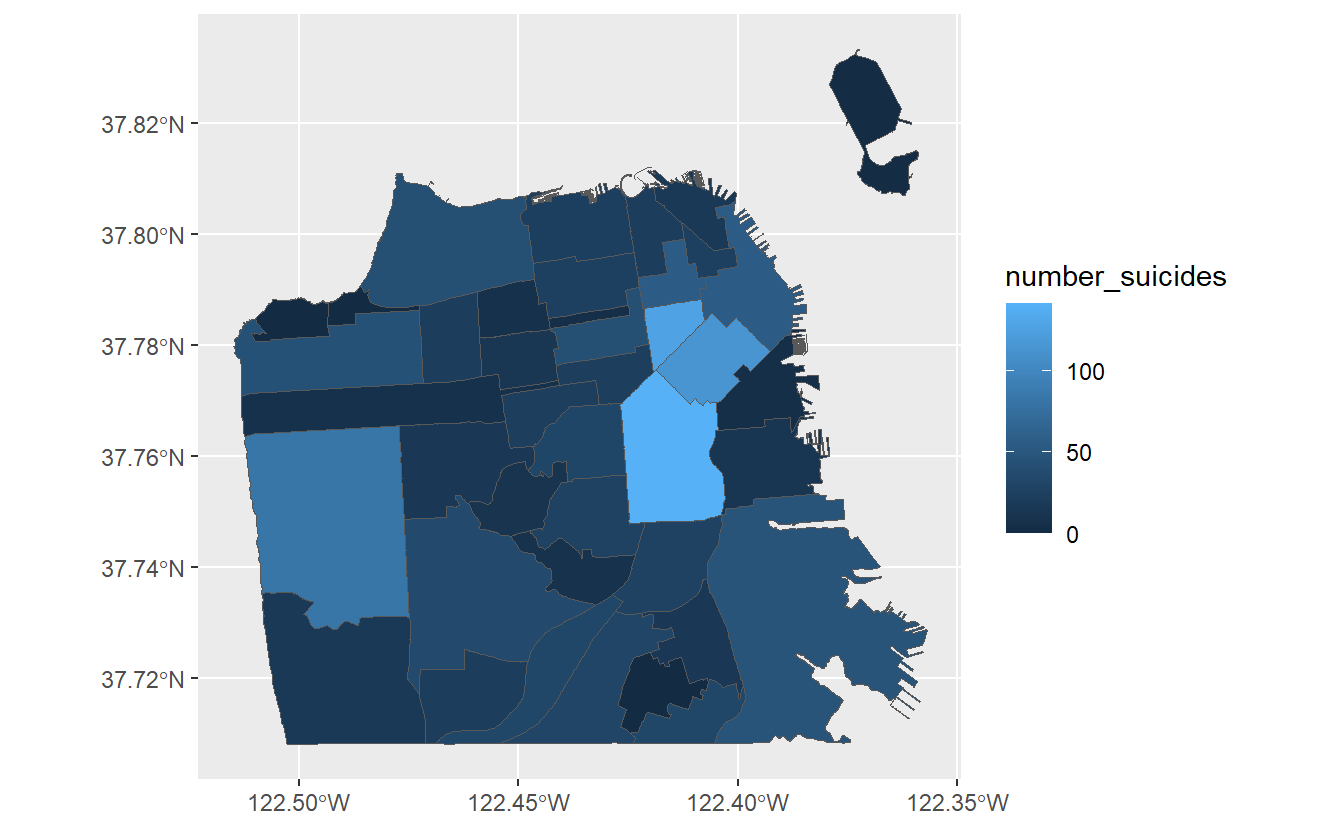
\includegraphics[width=1\linewidth,height=0.45\textheight,]{crimebythenumbers_files/figure-latex/unnamed-chunk-26-1}

Finally, we can add a title to the legend using the
\texttt{title} parameter inside of \texttt{addLegend()}.

\begin{Shaded}
\begin{Highlighting}[]
\NormalTok{pal }\OtherTok{\textless{}{-}} \FunctionTok{colorNumeric}\NormalTok{(}\StringTok{"OrRd"}\NormalTok{, sf\_neighborhoods\_suicide}\SpecialCharTok{$}\NormalTok{number\_suicides)}
\FunctionTok{leaflet}\NormalTok{() }\SpecialCharTok{\%\textgreater{}\%}
  \FunctionTok{addTiles}\NormalTok{(}\StringTok{"http://\{s\}.tile.openstreetmap.org/\{z\}/\{x\}/\{y\}.png"}\NormalTok{,}
    \AttributeTok{attribution =} \StringTok{\textquotesingle{}\&copy; \textless{}a href="http://openstreetmap.org"\textgreater{}}
\StringTok{                OpenStreetMap\textless{}/a\textgreater{} contributors\textquotesingle{}}
\NormalTok{  ) }\SpecialCharTok{\%\textgreater{}\%}
  \FunctionTok{addPolygons}\NormalTok{(}
    \AttributeTok{data =}\NormalTok{ sf\_neighborhoods\_suicide}\SpecialCharTok{$}\NormalTok{geometry,}
    \AttributeTok{col =} \StringTok{"black"}\NormalTok{,}
    \AttributeTok{weight =} \DecValTok{1}\NormalTok{,}
    \AttributeTok{popup =} \FunctionTok{paste0}\NormalTok{(}
      \StringTok{"Neighborhood: "}\NormalTok{,}
\NormalTok{      sf\_neighborhoods\_suicide}\SpecialCharTok{$}\NormalTok{nhood,}
      \StringTok{"\textless{}br\textgreater{}"}\NormalTok{,}
      \StringTok{"Number of Suicides: "}\NormalTok{,}
\NormalTok{      sf\_neighborhoods\_suicide}\SpecialCharTok{$}\NormalTok{number\_suicides}
\NormalTok{    ),}
    \AttributeTok{fillColor =} \FunctionTok{pal}\NormalTok{(sf\_neighborhoods\_suicide}\SpecialCharTok{$}\NormalTok{number\_suicides),}
    \AttributeTok{fillOpacity =} \DecValTok{1}
\NormalTok{  ) }\SpecialCharTok{\%\textgreater{}\%}
  \FunctionTok{addLegend}\NormalTok{(}
    \AttributeTok{pal =}\NormalTok{ pal,}
    \AttributeTok{values =}\NormalTok{ sf\_neighborhoods\_suicide}\SpecialCharTok{$}\NormalTok{number\_suicides,}
    \AttributeTok{opacity =} \DecValTok{1}\NormalTok{,}
    \AttributeTok{title =} \StringTok{"Suicides"}
\NormalTok{  )}
\end{Highlighting}
\end{Shaded}

\textbackslash begin\{center\}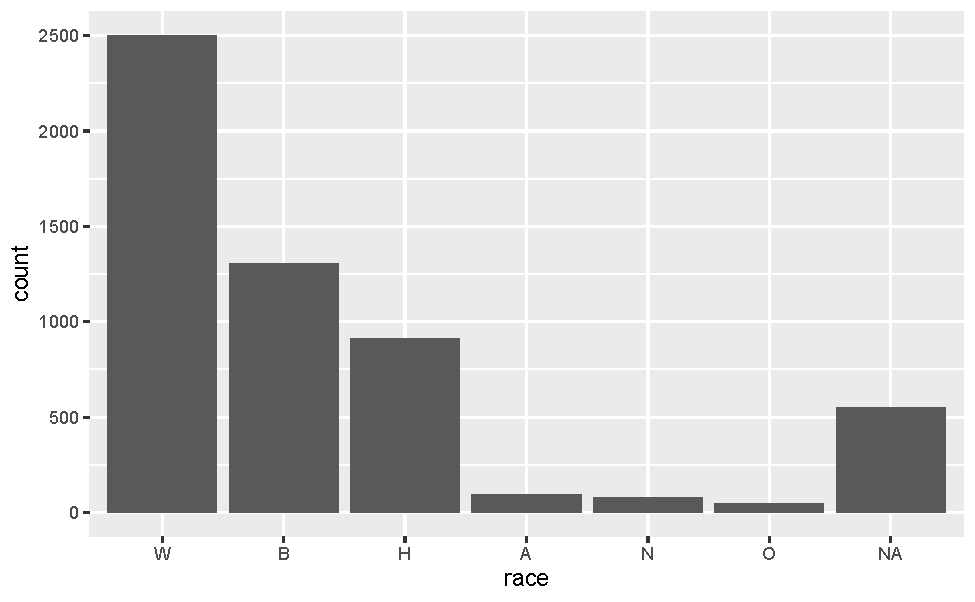
\includegraphics[width=1\linewidth,height=0.45\textheight,]{crimebythenumbers_files/figure-latex/unnamed-chunk-27-1}

\hypertarget{scrape-table}{%
\chapter{Scraping tables from PDFs}\label{scrape-table}}

For this chapter you'll need the following file, which is
available for download
\href{https://github.com/jacobkap/r4crimz/tree/master/data}{here}:
usbp\_stats\_fy2017\_sector\_profile.pdf.

Government agencies in particular like to release their data
in long PDFs which often have the data we want in a table on
one of the pages. To use this data we need to scrape it from
the PDF into R. In the majority of cases when you want data
from a PDF it will be in a table. Essentially the data will
be an Excel file inside of a PDF. This format is not
altogether different than what we've done before.

Let's first take a look at the data we will be scraping. The
first step in any PDF scraping should be to look at the PDF
and try to think about the best way to approach this
particular problem. While all PDF scraping follows a general
format, you cannot necessarily reuse your old code as each
situation is likely slightly different. Our data is from the
US Customs and Border Protection (CBP) and contains a wealth
of information about apprehensions and contraband seizures
in border sectors.

We will be using the Sector Profile 2017 PDF which has
information in four tables, three of which we'll scrape and
then combine together. The data was downloaded from the US
Customs and Border Protection ``Stats and Summaries'' page
\href{https://www.cbp.gov/newsroom/media-resources/stats}{here}.
If you're interested in using more of their data, some of it
has been cleaned and made available
\href{https://www.openicpsr.org/openicpsr/project/109522/version/V2/view}{here}.

The file we want to use is called
``usbp\_stats\_fy2017\_sector\_profile.pdf'' and has four
tables in the PDF. Let's take a look at them one at a time,
understanding what variables are available, and what units
each row is in. Then we'll start scraping the tables.

The first table is ``Sector Profile - Fiscal Year 2017
(Oct.~1st through Sept.~30th)''. Before we even look down
more at the table, the title is important. It is for fiscal
year 2017, not calendar year 2017 which is more common in
the data we usually use. This is important if we ever want
to merge this data with other data sets. If possible, we
would have to get data that is monthly so we can just use
October 2016 through September 2017 to match up properly.

\begin{center}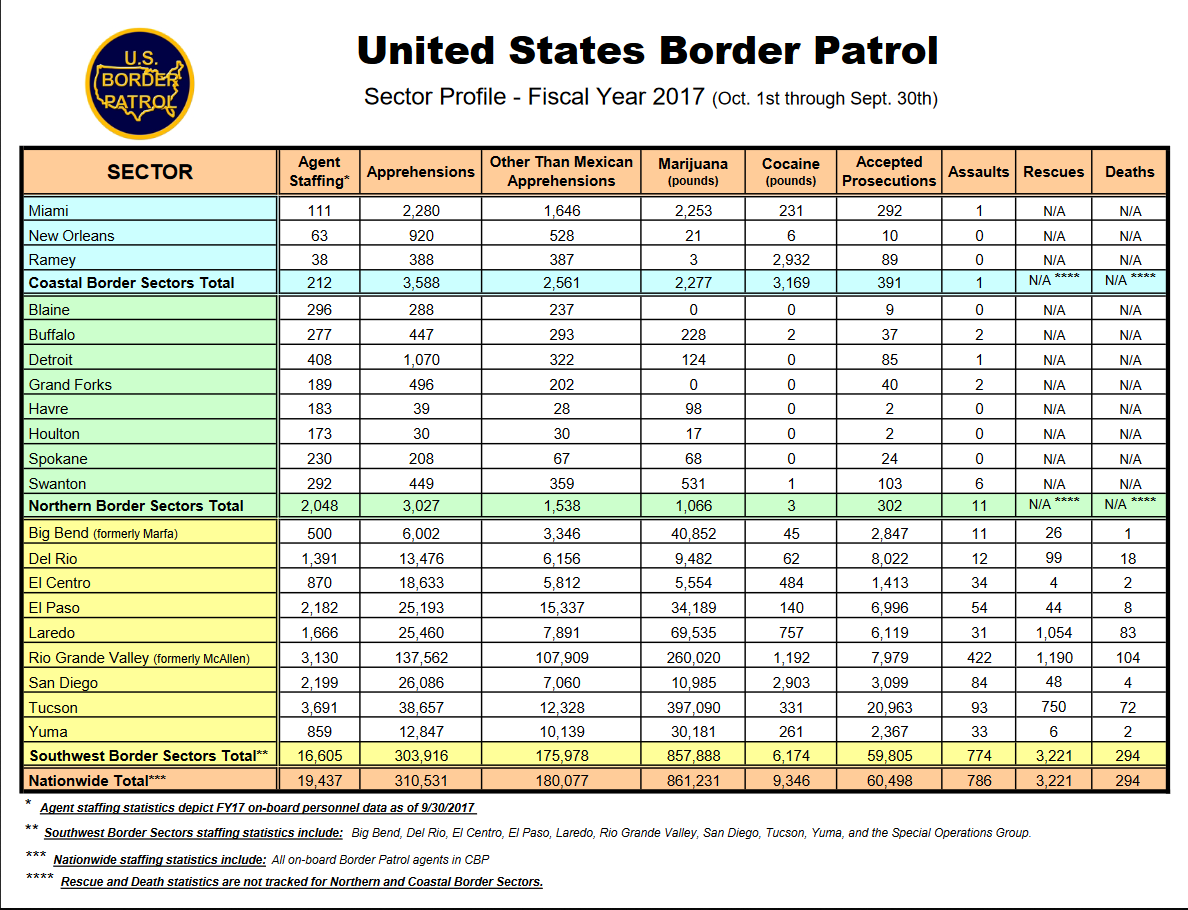
\includegraphics[width=1\linewidth,height=0.45\textheight,]{images/pdf_table_1} \end{center}

Now if we look more at the table, we can see that each row
is a section of the US border. There are three main sections
- Coastal, Northern, and Southwest, with subsections of each
also included. The bottom row is the sum of all these
sections and gives us nationwide data. Many government data
sets will be like this form with sections and subsections in
the same table. Watch out when doing mathematical
operations! Just summing any of these columns will give you
triple the true value due to the presence of nationwide,
sectional, and subsectional data.

There are 9 columns in the data other than the border
section identifier. We have total apprehensions,
apprehensions for people who are not Mexican citizens,
marijuana and cocaine seizures (in pounds), the number of
accepted prosecutions (presumably of those apprehended), and
the number of CBP agents assaulted. The last two columns
have the number of people rescued by CBP and the number of
people who died (it is unclear from this data alone if this
is solely people in custody or deaths during crossing the
border). These two columns are also special as they only
have data for the Southwest border.

Table 2 has a similar format with each row being a section
or subsection. The columns now have the number of juveniles
apprehended, subdivided by if they were accompanied by an
adult or not, and the number of adults apprehended. The last
column is total apprehensions which is also in Table 1.

\begin{center}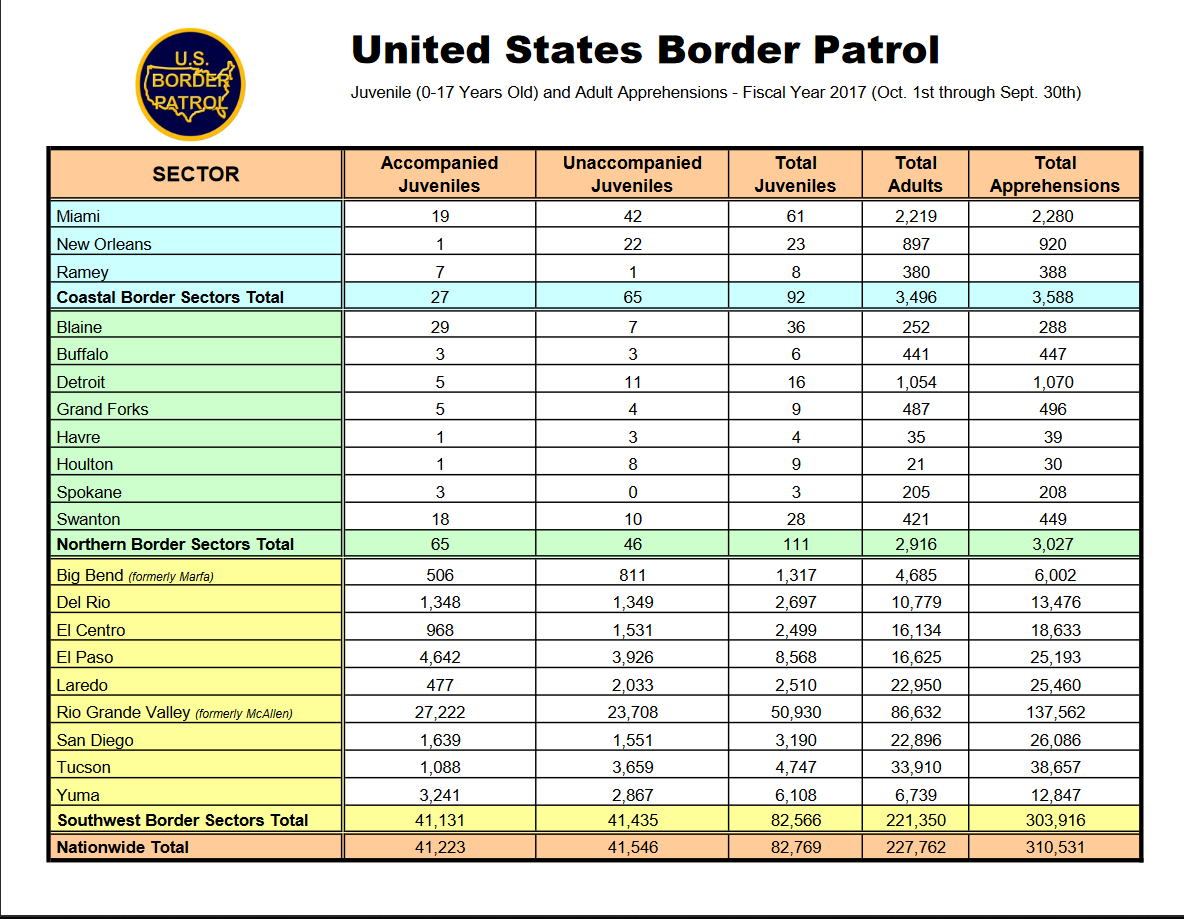
\includegraphics[width=1\linewidth,height=0.45\textheight,]{images/pdf_table_2} \end{center}

Table 3 follows the same format and the new columns are
number of apprehensions by gender.

\begin{center}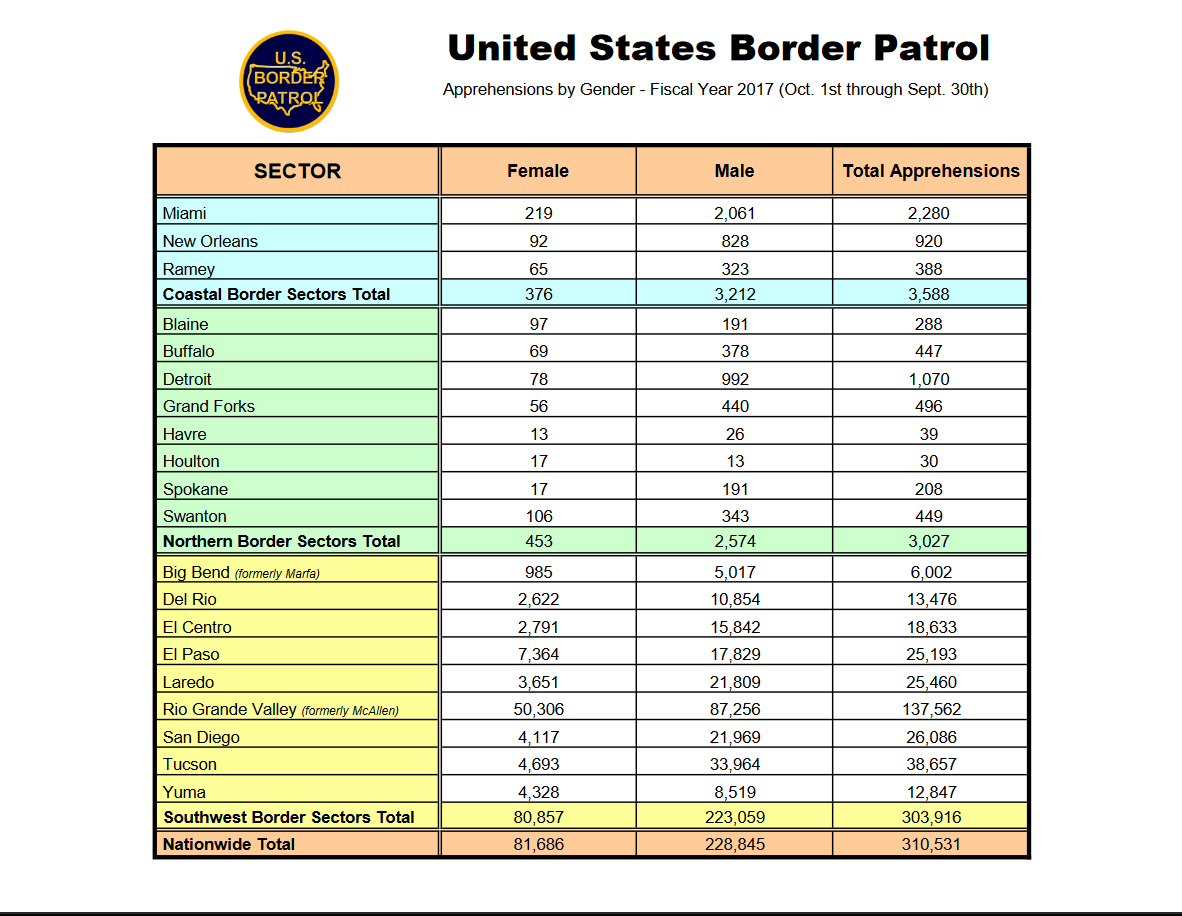
\includegraphics[width=1\linewidth,height=0.45\textheight,]{images/pdf_table_3} \end{center}

Finally, Table 4 is a bit different in its format. The rows
are now variables and the columns are the locations. In this
table it doesn't include subsections, only border sections
and the nationwide total. The data it has available are
partially a repeat of Table 1 but with more drug types and
the addition of the number of drug seizures and some firearm
seizure information. As this table is formatted differently
than the others, we won't scrape it in this lesson - but you
can use the skills you'll learn to do so yourself.

\begin{center}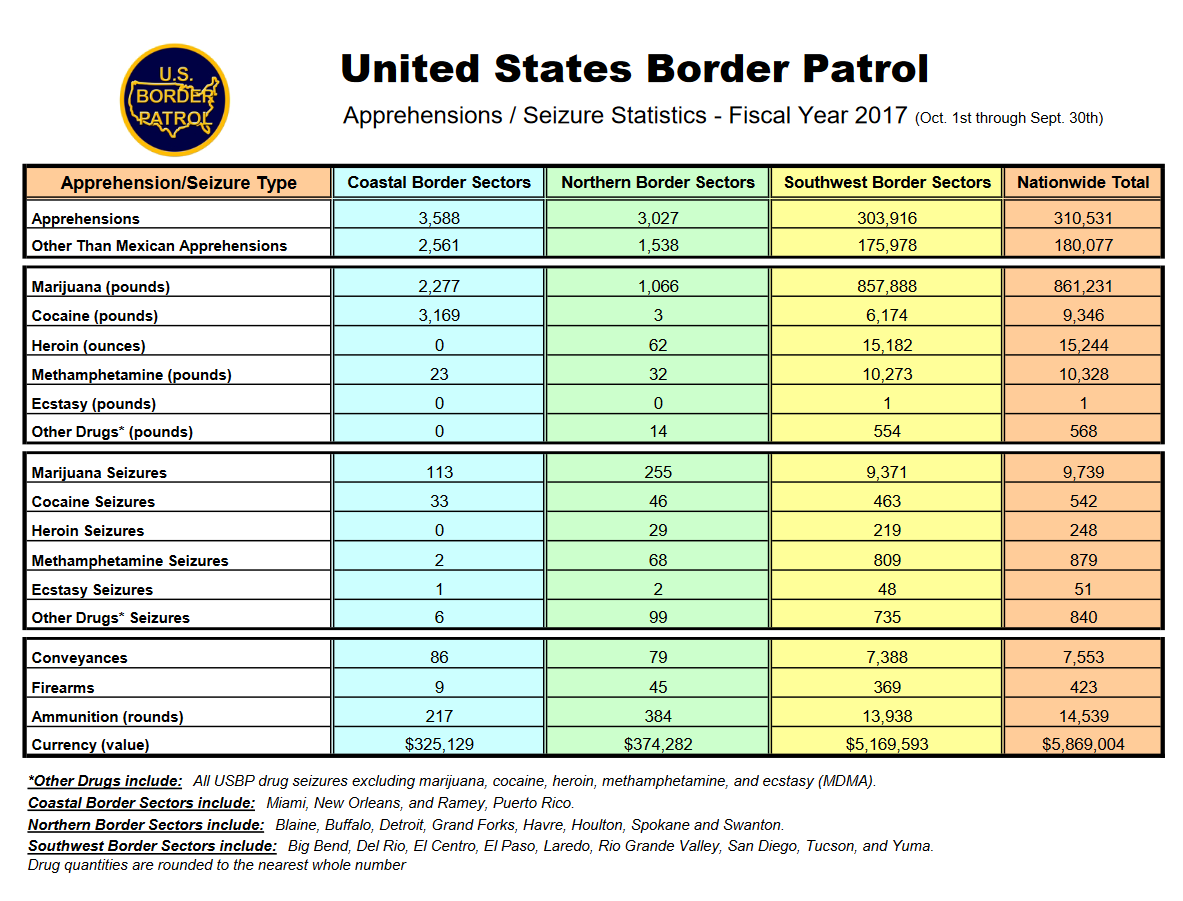
\includegraphics[width=1\linewidth,height=0.45\textheight,]{images/pdf_table_4} \end{center}

\hypertarget{scraping-the-first-table}{%
\section{Scraping the first
table}\label{scraping-the-first-table}}

We've now seen all three of the tables that we want to
scrape so we can begin the process of actually scraping
them. Note that each table is very similar meaning that we
can reuse some code to scrape as well as to clean the data.
That means that we will want to write some functions to make
our work easier and avoid copy and pasting code.

We will start by using the \texttt{pdf\_text()} function
from the \texttt{pdftools} package to read the PDFs into R.

\begin{Shaded}
\begin{Highlighting}[]
\FunctionTok{install.packages}\NormalTok{(}\StringTok{"pdftools"}\NormalTok{)}
\end{Highlighting}
\end{Shaded}

\begin{Shaded}
\begin{Highlighting}[]
\FunctionTok{library}\NormalTok{(pdftools)}
\end{Highlighting}
\end{Shaded}

We can assign the output of the \texttt{pdf\_text()}
function to the object \emph{border\_patrol} and we'll use
it for each table. The input to \texttt{pdf\_text()} is the
name of the PDF we want to scrape.

\begin{Shaded}
\begin{Highlighting}[]
\NormalTok{border\_patrol }\OtherTok{\textless{}{-}} \FunctionTok{pdf\_text}\NormalTok{(}\StringTok{"data/usbp\_stats\_fy2017\_sector\_profile.pdf"}\NormalTok{)}
\end{Highlighting}
\end{Shaded}

We can take a look at the \texttt{head()} of the result.

\begin{Shaded}
\begin{Highlighting}[]
\FunctionTok{head}\NormalTok{(border\_patrol)}
\end{Highlighting}
\end{Shaded}

{[}1{]} '' United States Border
Patrol\n                                                            Sector
Profile - Fiscal Year 2017 (Oct.~1st through
Sept.~30th)\n\n                                                Agent
Other Than Mexican Marijuana Cocaine
Accepted\n              SECTOR
Staffing\emph{\n                                                             Apprehensions\n                                                                                     Apprehensions
(pounds) (pounds)
Prosecutions\n                                                                                                                                                               Assaults
Rescues
Deaths\n\nMiami                                             111
2,280 1,646 2,253 231 292 1 N/A N/A\nNew Orleans 63 920 528
21 6 10 0 N/A
N/A\nRamey                                              38
388 387 3 2,932 89 0 N/A N/A\nCoastal Border Sectors Total
212 3,588 2,561 2,277 3,169 391 1 N/A }*** N/A
****\n\nBlaine                                            296
288 237 0 0 9 0 N/A
N/A\nBuffalo                                           277
447 293 228 2 37 2 N/A
N/A\nDetroit                                           408
1,070 322 124 0 85 1 N/A N/A\nGrand Forks 189 496 202 0 0 40
2 N/A
N/A\nHavre                                             183
39 28 98 0 2 0 N/A
N/A\nHoulton                                           173
30 30 17 0 2 0 N/A
N/A\nSpokane                                           230
208 67 68 0 24 0 N/A
N/A\nSwanton                                           292
449 359 531 1 103 6 N/A N/A\nNorthern Border Sectors Total
2,048 3,027 1,538 1,066 3 302 11 N/A **** N/A ****\nBig Bend
(formerly Marfa) 500 6,002 3,346 40,852 45 2,847 11 26
1\nDel Rio 1,391 13,476 6,156 9,482 62 8,022 12 99
18\nEl Centro 870 18,633 5,812 5,554 484 1,413 34 4
2\nEl Paso 2,182 25,193 15,337 34,189 140 6,996 54 44
8\nLaredo                                           1,666
25,460 7,891 69,535 757 6,119 31 1,054 83\nRio Grande Valley
(formerly McAllen) 3,130 137,562 107,909 260,020 1,192 7,979
422 1,190 104\nSan Diego 2,199 26,086 7,060 10,985 2,903
3,099 84 48
4\nTucson                                           3,691
38,657 12,328 397,090 331 20,963 93 750
72\nYuma                                              859
12,847 10,139 30,181 261 2,367 33 6 2\nSouthwest Border
Sectors Total** 16,605 303,916 175,978 857,888 6,174 59,805
774 3,221 294\nNationwide Total*** 19,437 310,531 180,077
861,231 9,346 60,498 786 3,221 294\n* Agent staffing
statistics depict FY17 on-board personnel data as of
9/30/2017\n** Southwest Border Sectors staffing statistics
include: Big Bend, Del Rio, El Centro, El Paso, Laredo, Rio
Grande Valley, San Diego, Tucson, Yuma, and the Special
Operations Group.\n*** Nationwide staffing statistics
include: All on-board Border Patrol agents in CBP\n****
Rescue and Death statistics are not tracked for Northern and
Coastal Border Sectors.\n'' {[}2{]} '' United States Border
Patrol\n                                       Juvenile
(0-17 Years Old) and Adult Apprehensions - Fiscal Year 2017
(Oct.~1st through
Sept.~30th)\n\n\n\n                                           Accompanied
Unaccompanied Total Total Total\n               SECTOR
Juveniles Juveniles Juveniles Adults
Apprehensions\nMiami                                            19
42 61 2,219 2,280\nNew Orleans 1 22 23 897
920\nRamey                                             7 1 8
380 388\nCoastal Border Sectors Total 27 65 92 3,496
3,588\nBlaine                                           29 7
36 252
288\nBuffalo                                           3 3 6
441 447\nDetroit                                           5
11 16 1,054 1,070\nGrand Forks 5 4 9 487
496\nHavre                                             1 3 4
35 39\nHoulton                                           1 8
9 21 30\nSpokane                                           3
0 3 205
208\nSwanton                                          18 10
28 421 449\nNorthern Border Sectors Total 65 46 111 2,916
3,027\nBig Bend (formerly Marfa) 506 811 1,317 4,685
6,002\nDel Rio 1,348 1,349 2,697 10,779 13,476\nEl Centro
968 1,531 2,499 16,134 18,633\nEl Paso 4,642 3,926 8,568
16,625
25,193\nLaredo                                           477
2,033 2,510 22,950 25,460\nRio Grande Valley (formerly
McAllen) 27,222 23,708 50,930 86,632 137,562\nSan Diego
1,639 1,551 3,190 22,896
26,086\nTucson                                          1,088
3,659 4,747 33,910
38,657\nYuma                                            3,241
2,867 6,108 6,739 12,847\nSouthwest Border Sectors Total
41,131 41,435 82,566 221,350 303,916\nNationwide Total
41,223 41,546 82,769 227,762 310,531\n''\\
{[}3{]} '' United States Border
Patrol\n                                       Apprehensions
by Gender - Fiscal Year 2017 (Oct.~1st through
Sept.~30th)\n\n\n\n\n              SECTOR Female Male Total
Apprehensions\n\nMiami                                            219
2,061 2,280\nNew Orleans 92 828
920\nRamey                                             65
323 388\nCoastal Border Sectors Total 376 3,212
3,588\nBlaine                                            97
191
288\nBuffalo                                           69
378
447\nDetroit                                           78
992 1,070\nGrand Forks 56 440
496\nHavre                                             13 26
39\nHoulton                                           17 13
30\nSpokane                                           17 191
208\nSwanton                                          106
343 449\nNorthern Border Sectors Total 453 2,574
3,027\nBig Bend (formerly Marfa) 985 5,017 6,002\nDel Rio
2,622 10,854 13,476\nEl Centro 2,791 15,842 18,633\nEl Paso
7,364 17,829
25,193\nLaredo                                          3,651
21,809 25,460\nRio Grande Valley (formerly McAllen) 50,306
87,256 137,562\nSan Diego 4,117 21,969
26,086\nTucson                                          4,693
33,964
38,657\nYuma                                            4,328
8,519 12,847\nSouthwest Border Sectors Total 80,857 223,059
303,916\nNationwide Total 81,686 228,845 310,531\n''\\
{[}4{]} '' United States Border
Patrol\n                                            Apprehensions
/ Seizure Statistics - Fiscal Year 2017 (Oct.~1st through
Sept.~30th)\n\n    Apprehension/Seizure Type Coastal Border
Sectors Northern Border Sectors Southwest Border Sectors
Nationwide
Total\n\nApprehensions                                          3,588
3,027 303,916 310,531\nOther Than Mexican Apprehensions
2,561 1,538 175,978 180,077\n\nMarijuana (pounds) 2,277
1,066 857,888 861,231\nCocaine (pounds) 3,169 3 6,174
9,346\nHeroin (ounces) 0 62 15,182
15,244\nMethamphetamine (pounds) 23 32 10,273
10,328\nEcstasy (pounds) 0 0 1 1\nOther Drugs* (pounds) 0 14
554 568\n\nMarijuana Seizures 113 255 9,371
9,739\nCocaine Seizures 33 46 463 542\nHeroin Seizures 0 29
219 248\nMethamphetamine Seizures 2 68 809
879\nEcstasy Seizures 1 2 48 51\nOther Drugs* Seizures 6 99
735
840\n\nConveyances                                             86
79 7,388
7,553\nFirearms                                                 9
45 369 423\nAmmunition (rounds) 217 384 13,938
14,539\nCurrency (value) \$325,129 \$374,282 \$5,169,593
\$5,869,004\n\n*Other Drugs include: All USBP drug seizures
excluding marijuana, cocaine, heroin, methamphetamine, and
ecstasy (MDMA).\nCoastal Border Sectors include: Miami, New
Orleans, and Ramey, Puerto Rico.\nNorthern Border Sectors
include: Blaine, Buffalo, Detroit, Grand Forks, Havre,
Houlton, Spokane and Swanton.\nSouthwest Border Sectors
include: Big Bend, Del Rio, El Centro, El Paso, Laredo, Rio
Grande Valley, San Diego, Tucson, and Yuma.\nDrug quantities
are rounded to the nearest whole number\n''

If you look closely in this huge amount of text output, you
can see that it is a vector with each table being an element
in the vector. We can see this further by checking the
\texttt{length()} of ``border\_patrol'' which tells us how
many elements are in a vector.

\begin{Shaded}
\begin{Highlighting}[]
\FunctionTok{length}\NormalTok{(border\_patrol)}
\end{Highlighting}
\end{Shaded}

{[}1{]} 4

It is four elements long, one for each table.

Looking at just the first element in \emph{border\_patrol}
gives us all the values in the first table plus a few
sentences at the end detailing some features of the table.
At the end of each line (where in the PDF it should end but
doesn't in our data yet) there is a
\texttt{\textbackslash{}n} indicating that there should be a
new line. We want to use \texttt{strsplit()} to split at the
\texttt{\textbackslash{}n}.

\begin{Shaded}
\begin{Highlighting}[]
\NormalTok{border\_patrol[}\DecValTok{1}\NormalTok{]}
\end{Highlighting}
\end{Shaded}

{[}1{]} '' United States Border
Patrol\n                                                            Sector
Profile - Fiscal Year 2017 (Oct.~1st through
Sept.~30th)\n\n                                                Agent
Other Than Mexican Marijuana Cocaine
Accepted\n              SECTOR
Staffing\emph{\n                                                             Apprehensions\n                                                                                     Apprehensions
(pounds) (pounds)
Prosecutions\n                                                                                                                                                               Assaults
Rescues
Deaths\n\nMiami                                             111
2,280 1,646 2,253 231 292 1 N/A N/A\nNew Orleans 63 920 528
21 6 10 0 N/A
N/A\nRamey                                              38
388 387 3 2,932 89 0 N/A N/A\nCoastal Border Sectors Total
212 3,588 2,561 2,277 3,169 391 1 N/A }*** N/A
****\n\nBlaine                                            296
288 237 0 0 9 0 N/A
N/A\nBuffalo                                           277
447 293 228 2 37 2 N/A
N/A\nDetroit                                           408
1,070 322 124 0 85 1 N/A N/A\nGrand Forks 189 496 202 0 0 40
2 N/A
N/A\nHavre                                             183
39 28 98 0 2 0 N/A
N/A\nHoulton                                           173
30 30 17 0 2 0 N/A
N/A\nSpokane                                           230
208 67 68 0 24 0 N/A
N/A\nSwanton                                           292
449 359 531 1 103 6 N/A N/A\nNorthern Border Sectors Total
2,048 3,027 1,538 1,066 3 302 11 N/A **** N/A ****\nBig Bend
(formerly Marfa) 500 6,002 3,346 40,852 45 2,847 11 26
1\nDel Rio 1,391 13,476 6,156 9,482 62 8,022 12 99
18\nEl Centro 870 18,633 5,812 5,554 484 1,413 34 4
2\nEl Paso 2,182 25,193 15,337 34,189 140 6,996 54 44
8\nLaredo                                           1,666
25,460 7,891 69,535 757 6,119 31 1,054 83\nRio Grande Valley
(formerly McAllen) 3,130 137,562 107,909 260,020 1,192 7,979
422 1,190 104\nSan Diego 2,199 26,086 7,060 10,985 2,903
3,099 84 48
4\nTucson                                           3,691
38,657 12,328 397,090 331 20,963 93 750
72\nYuma                                              859
12,847 10,139 30,181 261 2,367 33 6 2\nSouthwest Border
Sectors Total** 16,605 303,916 175,978 857,888 6,174 59,805
774 3,221 294\nNationwide Total*** 19,437 310,531 180,077
861,231 9,346 60,498 786 3,221 294\n* Agent staffing
statistics depict FY17 on-board personnel data as of
9/30/2017\n** Southwest Border Sectors staffing statistics
include: Big Bend, Del Rio, El Centro, El Paso, Laredo, Rio
Grande Valley, San Diego, Tucson, Yuma, and the Special
Operations Group.\n*** Nationwide staffing statistics
include: All on-board Border Patrol agents in CBP\n****
Rescue and Death statistics are not tracked for Northern and
Coastal Border Sectors.\n''

The \texttt{strsplit()} function breaks up a string into
pieces based on a value inside of the string. Let's use the
word ``criminology'' as an example. If we want to split it
by the letter ``n'' we'd have two results, ``crimi'' and
``ology'' as these are the pieces of the word after breaking
up ``criminology'' at letter ``n''.

\begin{Shaded}
\begin{Highlighting}[]
\FunctionTok{strsplit}\NormalTok{(}\StringTok{"criminology"}\NormalTok{, }\AttributeTok{split =} \StringTok{"n"}\NormalTok{)}
\CommentTok{\#\textgreater{} [[1]]}
\CommentTok{\#\textgreater{} [1] "crimi" "ology"}
\end{Highlighting}
\end{Shaded}

Note that it deletes whatever value is used to break up the
string.

Let's assign a new object with the value in the first
element of \emph{border\_patrol}, calling it
\emph{sector\_profile} as that's the name of that table, and
then using \texttt{strsplit()} on it to split it every
\texttt{\textbackslash{}n}. In effect this makes each line
of the table an element in a vector that we'll create rather
than having the entire table be a single long string as it
is now. \texttt{strsplit()} returns a list so we will also
want to keep just the first element of that list using
double square bracket \texttt{{[}{[}{]}{]}} notation.

\begin{Shaded}
\begin{Highlighting}[]
\NormalTok{sector\_profile }\OtherTok{\textless{}{-}}\NormalTok{ border\_patrol[}\DecValTok{1}\NormalTok{]}
\NormalTok{sector\_profile }\OtherTok{\textless{}{-}} \FunctionTok{strsplit}\NormalTok{(sector\_profile, }\StringTok{"}\SpecialCharTok{\textbackslash{}n}\StringTok{"}\NormalTok{)}
\NormalTok{sector\_profile }\OtherTok{\textless{}{-}}\NormalTok{ sector\_profile[[}\DecValTok{1}\NormalTok{]]}
\end{Highlighting}
\end{Shaded}

Now we can look at the first six rows of this data.

\begin{Shaded}
\begin{Highlighting}[]
\FunctionTok{head}\NormalTok{(sector\_profile)}
\end{Highlighting}
\end{Shaded}

{[}1{]} '' United States Border Patrol''\\
{[}2{]} '' Sector Profile - Fiscal Year 2017 (Oct.~1st
through Sept.~30th)''\\
{[}3{]} ``\,''\\
{[}4{]} '' Agent Other Than Mexican Marijuana Cocaine
Accepted'' {[}5{]} '' SECTOR Staffing*''\\
{[}6{]} '' Apprehensions''

Notice that there is a lot of empty white space at the
beginning of the rows. We want to get rid of that to make
our next steps easier. We can use \texttt{trimws()} and put
the entire \emph{sector\_profile} data in the () and it'll
remove any white space that is at the beginning or end of
the string.

\begin{Shaded}
\begin{Highlighting}[]
\NormalTok{sector\_profile }\OtherTok{\textless{}{-}} \FunctionTok{trimws}\NormalTok{(sector\_profile)}
\end{Highlighting}
\end{Shaded}

We have more rows than we want so let's look at the entire
data and try to figure out how to keep just the necessary
rows.

\begin{Shaded}
\begin{Highlighting}[]
\NormalTok{sector\_profile}
\end{Highlighting}
\end{Shaded}

{[}1{]} ``United States Border Patrol''\\
{[}2{]} ``Sector Profile - Fiscal Year 2017 (Oct.~1st
through Sept.~30th)''\\
{[}3{]} ``\,''\\
{[}4{]} ``Agent Other Than Mexican Marijuana Cocaine
Accepted''\\
{[}5{]} ``SECTOR Staffing\emph{''\\
{[}6{]} ''Apprehensions''\\
{[}7{]} ''Apprehensions (pounds) (pounds) Prosecutions''\\
{[}8{]} ''Assaults Rescues Deaths''\\
{[}9{]} ''\,''\\
{[}10{]} ''Miami 111 2,280 1,646 2,253 231 292 1 N/A N/A''\\
{[}11{]} ''New Orleans 63 920 528 21 6 10 0 N/A N/A''\\
{[}12{]} ''Ramey 38 388 387 3 2,932 89 0 N/A N/A''\\
{[}13{]} ''Coastal Border Sectors Total 212 3,588 2,561
2,277 3,169 391 1 N/A }*** N/A ****''\\
{[}14{]} ``\,''\\
{[}15{]} ``Blaine 296 288 237 0 0 9 0 N/A N/A''\\
{[}16{]} ``Buffalo 277 447 293 228 2 37 2 N/A N/A''\\
{[}17{]} ``Detroit 408 1,070 322 124 0 85 1 N/A N/A''\\
{[}18{]} ``Grand Forks 189 496 202 0 0 40 2 N/A N/A''\\
{[}19{]} ``Havre 183 39 28 98 0 2 0 N/A N/A''\\
{[}20{]} ``Houlton 173 30 30 17 0 2 0 N/A N/A''\\
{[}21{]} ``Spokane 230 208 67 68 0 24 0 N/A N/A''\\
{[}22{]} ``Swanton 292 449 359 531 1 103 6 N/A N/A''\\
{[}23{]} ``Northern Border Sectors Total 2,048 3,027 1,538
1,066 3 302 11 N/A **** N/A ****'' {[}24{]} ``Big Bend
(formerly Marfa) 500 6,002 3,346 40,852 45 2,847 11 26 1''\\
{[}25{]} ``Del Rio 1,391 13,476 6,156 9,482 62 8,022 12 99
18''\\
{[}26{]} ``El Centro 870 18,633 5,812 5,554 484 1,413 34 4
2''\\
{[}27{]} ``El Paso 2,182 25,193 15,337 34,189 140 6,996 54
44 8''\\
{[}28{]} ``Laredo 1,666 25,460 7,891 69,535 757 6,119 31
1,054 83''\\
{[}29{]} ``Rio Grande Valley (formerly McAllen) 3,130
137,562 107,909 260,020 1,192 7,979 422 1,190 104''\\
{[}30{]} ``San Diego 2,199 26,086 7,060 10,985 2,903 3,099
84 48 4''\\
{[}31{]} ``Tucson 3,691 38,657 12,328 397,090 331 20,963 93
750 72''\\
{[}32{]} ``Yuma 859 12,847 10,139 30,181 261 2,367 33 6
2''\\
{[}33{]} ``Southwest Border Sectors Total** 16,605 303,916
175,978 857,888 6,174 59,805 774 3,221 294''\\
{[}34{]} ``Nationwide Total*** 19,437 310,531 180,077
861,231 9,346 60,498 786 3,221 294''\\
{[}35{]} ``* Agent staffing statistics depict FY17 on-board
personnel data as of 9/30/2017''\\
{[}36{]} ``** Southwest Border Sectors staffing statistics
include: Big Bend, Del Rio, El Centro, El Paso, Laredo, Rio
Grande Valley, San Diego, Tucson, Yuma, and the Special
Operations Group.''\\
{[}37{]} ``*** Nationwide staffing statistics include: All
on-board Border Patrol agents in CBP''\\
{[}38{]} ``**** Rescue and Death statistics are not tracked
for Northern and Coastal Border Sectors.''

Based on the PDF, we want every row from Miami to Nationwide
Total. But here we have several rows with the title of the
table and the column names, and at the end we have the
sentences with some details that we don't need.

To keep only the rows that we want, we can combine
\texttt{grep()} and subsetting to find the rows from Miami
to Nationwide Total and keep only those rows. We will use
\texttt{grep()} to find which row has the text ``Miami'' and
which has the text ``Nationwide Total'' and keep all rows
between them (including those matched rows as well). Since
each only appears once in the table we don't need to worry
about handling duplicate results.

\begin{Shaded}
\begin{Highlighting}[]
\FunctionTok{grep}\NormalTok{(}\StringTok{"Miami"}\NormalTok{, sector\_profile)}
\CommentTok{\#\textgreater{} [1] 10}
\end{Highlighting}
\end{Shaded}

\begin{Shaded}
\begin{Highlighting}[]
\FunctionTok{grep}\NormalTok{(}\StringTok{"Nationwide Total"}\NormalTok{, sector\_profile)}
\CommentTok{\#\textgreater{} [1] 34}
\end{Highlighting}
\end{Shaded}

We'll use square bracket notation to keep all rows between
those two values (including each value). Since the data is a
vector, not a data.frame, we don't need a comma.

\begin{Shaded}
\begin{Highlighting}[]
\NormalTok{sector\_profile }\OtherTok{\textless{}{-}}\NormalTok{ sector\_profile[}\FunctionTok{grep}\NormalTok{(}\StringTok{"Miami"}\NormalTok{, sector\_profile)}\SpecialCharTok{:}\FunctionTok{grep}\NormalTok{(}\StringTok{"Nationwide Total"}\NormalTok{, sector\_profile)]}
\end{Highlighting}
\end{Shaded}

Note that we're getting rid of the rows which had the column
names. It's easier to make the names ourselves than to deal
with that mess. The data now has only the rows we want but
still doesn't have any columns, it's currently just a vector
of strings. We want to make it into a data.frame to be able
to work on it like we usually do.

\begin{Shaded}
\begin{Highlighting}[]
\FunctionTok{head}\NormalTok{(sector\_profile)}
\end{Highlighting}
\end{Shaded}

{[}1{]} ``Miami 111 2,280 1,646 2,253 231 292 1 N/A N/A''\\
{[}2{]} ``New Orleans 63 920 528 21 6 10 0 N/A N/A''\\
{[}3{]} ``Ramey 38 388 387 3 2,932 89 0 N/A N/A''\\
{[}4{]} ``Coastal Border Sectors Total 212 3,588 2,561 2,277
3,169 391 1 N/A **** N/A ****'' {[}5{]} ``\,''\\
{[}6{]} ``Blaine 296 288 237 0 0 9 0 N/A N/A''

When looking at this data it is clear that where the
division between columns is supposed to be is a bunch of
white space in each string. Take the first row for example,
it says ``Miami'' then after lots of white spaces ``111''
than again with ``2,280'' and so on for the rest of the row.
We'll use this pattern of columns differentiated by white
space to make \emph{sector\_profile} into a data.frame.

We will use the function \texttt{str\_split\_fixed()} from
the \texttt{stringr} package. This function is very similar
to \texttt{strsplit()} except you can tell it how many
columns to expect.

\begin{Shaded}
\begin{Highlighting}[]
\FunctionTok{install.packages}\NormalTok{(}\StringTok{"stringr"}\NormalTok{)}
\end{Highlighting}
\end{Shaded}

\begin{Shaded}
\begin{Highlighting}[]
\FunctionTok{library}\NormalTok{(stringr)}
\end{Highlighting}
\end{Shaded}

The syntax of \texttt{str\_split\_fixed()} is similar to
\texttt{strsplit()} except the new parameter of the number
of splits to expect. The ``\_fixed'' part of
\texttt{str\_split\_fixed()} is that it expects the same
number of splits (which in our case become columns) for
every element in the vector that we input. Looking at the
PDF shows us that there are 10 columns so that's the number
we'll use. Our split will be '' \{2,\}``. That is, a space
that occurs two or more times. Since there are sectors with
spaces in their name, we can't have only one space, we need
at least two. If you look carefully at the rows with
sectors''Coastal Border Sectors Total'' and ``Northern
Border Sectors Total'', the final two columns actually do
not have two spaces between them because of the amount of
asterisks they have. Normally we'd want to fix this using
\texttt{gsub()}, but those values will turn to NA anyway so
we won't bother in this case.

\begin{Shaded}
\begin{Highlighting}[]
\NormalTok{sector\_profile }\OtherTok{\textless{}{-}} \FunctionTok{str\_split\_fixed}\NormalTok{(sector\_profile, }\StringTok{" \{2,\}"}\NormalTok{, }\DecValTok{10}\NormalTok{)}
\end{Highlighting}
\end{Shaded}

If we check the \texttt{head()} we can see that we have the
proper columns now, but this still isn't a data.frame and
has no column names.

\begin{Shaded}
\begin{Highlighting}[]
\FunctionTok{head}\NormalTok{(sector\_profile)}
\end{Highlighting}
\end{Shaded}

\begin{verbatim}
 [,1]                           [,2]  [,3]    [,4]   
\end{verbatim}

{[}1,{]} ``Miami'' ``111'' ``2,280'' ``1,646'' {[}2,{]}
``New Orleans'' ``63'' ``920'' ``528''\\
{[}3,{]} ``Ramey'' ``38'' ``388'' ``387''\\
{[}4,{]} ``Coastal Border Sectors Total'' ``212'' ``3,588''
``2,561'' {[}5,{]} ``\,'' ``\,'' ``\,'' ``\,''\\
{[}6,{]} ``Blaine'' ``296'' ``288'' ``237''\\
{[},5{]} {[},6{]} {[},7{]} {[},8{]} {[},9{]} {[},10{]}\\
{[}1,{]} ``2,253'' ``231'' ``292'' ``1'' ``N/A'' ``N/A''\\
{[}2,{]} ``21'' ``6'' ``10'' ``0'' ``N/A'' ``N/A''\\
{[}3,{]} ``3'' ``2,932'' ``89'' ``0'' ``N/A'' ``N/A''\\
{[}4,{]} ``2,277'' ``3,169'' ``391'' ``1'' ``N/A ****''
``N/A ****'' {[}5,{]} ``\,'' ``\,'' ``\,'' ``\,'' ``\,''
``\,''\\
{[}6,{]} ``0'' ``0'' ``9'' ``0'' ``N/A'' ``N/A''

We can make it a data.frame just by putting it in
\texttt{data.frame()}. And we can assign the columns names
using a vector of strings we can make. We'll use the same
column names as in the PDF but in lowercase and replacing
spaces and parentheses with underscores.

\begin{Shaded}
\begin{Highlighting}[]
\NormalTok{sector\_profile }\OtherTok{\textless{}{-}} \FunctionTok{data.frame}\NormalTok{(sector\_profile)}
\FunctionTok{names}\NormalTok{(sector\_profile) }\OtherTok{\textless{}{-}} \FunctionTok{c}\NormalTok{(}
  \StringTok{"sector"}\NormalTok{,}
  \StringTok{"agent\_staffing"}\NormalTok{,}
  \StringTok{"apprehensions"}\NormalTok{,}
  \StringTok{"other\_than\_mexican\_apprehensions"}\NormalTok{,}
  \StringTok{"marijuana\_pounds"}\NormalTok{,}
  \StringTok{"cocaine\_pounds"}\NormalTok{,}
  \StringTok{"accepted\_prosecutions"}\NormalTok{,}
  \StringTok{"assaults"}\NormalTok{,}
  \StringTok{"rescues"}\NormalTok{,}
  \StringTok{"deaths"}
\NormalTok{)}
\end{Highlighting}
\end{Shaded}

We have now taken a table from a PDF and successfully
scraped it to a data.frame in R. Now we can work on it as we
would any other data set that we've used previously.

\begin{Shaded}
\begin{Highlighting}[]
\FunctionTok{head}\NormalTok{(sector\_profile)}
\CommentTok{\#\textgreater{}                         sector agent\_staffing apprehensions}
\CommentTok{\#\textgreater{} 1                        Miami            111         2,280}
\CommentTok{\#\textgreater{} 2                  New Orleans             63           920}
\CommentTok{\#\textgreater{} 3                        Ramey             38           388}
\CommentTok{\#\textgreater{} 4 Coastal Border Sectors Total            212         3,588}
\CommentTok{\#\textgreater{} 5                                                          }
\CommentTok{\#\textgreater{} 6                       Blaine            296           288}
\CommentTok{\#\textgreater{}   other\_than\_mexican\_apprehensions marijuana\_pounds}
\CommentTok{\#\textgreater{} 1                            1,646            2,253}
\CommentTok{\#\textgreater{} 2                              528               21}
\CommentTok{\#\textgreater{} 3                              387                3}
\CommentTok{\#\textgreater{} 4                            2,561            2,277}
\CommentTok{\#\textgreater{} 5                                                  }
\CommentTok{\#\textgreater{} 6                              237                0}
\CommentTok{\#\textgreater{}   cocaine\_pounds accepted\_prosecutions assaults  rescues}
\CommentTok{\#\textgreater{} 1            231                   292        1      N/A}
\CommentTok{\#\textgreater{} 2              6                    10        0      N/A}
\CommentTok{\#\textgreater{} 3          2,932                    89        0      N/A}
\CommentTok{\#\textgreater{} 4          3,169                   391        1 N/A ****}
\CommentTok{\#\textgreater{} 5                                                       }
\CommentTok{\#\textgreater{} 6              0                     9        0      N/A}
\CommentTok{\#\textgreater{}     deaths}
\CommentTok{\#\textgreater{} 1      N/A}
\CommentTok{\#\textgreater{} 2      N/A}
\CommentTok{\#\textgreater{} 3      N/A}
\CommentTok{\#\textgreater{} 4 N/A ****}
\CommentTok{\#\textgreater{} 5         }
\CommentTok{\#\textgreater{} 6      N/A}
\end{Highlighting}
\end{Shaded}

To really be able to use this data we'll want to clean the
columns to turn the values to numeric type but we can leave
that until later. For now let's write a function that
replicates much of this work for the next tables.

\hypertarget{making-a-function}{%
\section{Making a function}\label{making-a-function}}

As we've done before, we want to take the code we wrote for
the specific case of the first table in this PDF and turn it
into a function for the general case of other tables in the
PDF. Let's copy the code we used above before we convert it
to a function.

\begin{Shaded}
\begin{Highlighting}[]
\NormalTok{sector\_profile }\OtherTok{\textless{}{-}}\NormalTok{ border\_patrol[}\DecValTok{1}\NormalTok{]}
\NormalTok{sector\_profile }\OtherTok{\textless{}{-}} \FunctionTok{trimws}\NormalTok{(sector\_profile)}
\NormalTok{sector\_profile }\OtherTok{\textless{}{-}} \FunctionTok{strsplit}\NormalTok{(sector\_profile, }\StringTok{"}\SpecialCharTok{\textbackslash{}r\textbackslash{}n}\StringTok{"}\NormalTok{)}
\NormalTok{sector\_profile }\OtherTok{\textless{}{-}}\NormalTok{ sector\_profile[[}\DecValTok{1}\NormalTok{]]}
\NormalTok{sector\_profile }\OtherTok{\textless{}{-}}\NormalTok{ sector\_profile[}\FunctionTok{grep}\NormalTok{(}\StringTok{"Miami"}\NormalTok{, sector\_profile)}\SpecialCharTok{:}
\FunctionTok{grep}\NormalTok{(}\StringTok{"Nationwide Total"}\NormalTok{, sector\_profile)]}
\NormalTok{sector\_profile }\OtherTok{\textless{}{-}} \FunctionTok{str\_split\_fixed}\NormalTok{(sector\_profile, }\StringTok{" \{2,\}"}\NormalTok{, }\DecValTok{10}\NormalTok{)}
\NormalTok{sector\_profile }\OtherTok{\textless{}{-}} \FunctionTok{data.frame}\NormalTok{(sector\_profile)}
\FunctionTok{names}\NormalTok{(sector\_profile) }\OtherTok{\textless{}{-}} \FunctionTok{c}\NormalTok{(}
  \StringTok{"sector"}\NormalTok{,}
  \StringTok{"agent\_staffing"}\NormalTok{,}
  \StringTok{"total\_apprehensions"}\NormalTok{,}
  \StringTok{"other\_than\_mexican\_apprehensions"}\NormalTok{,}
  \StringTok{"marijuana\_pounds"}\NormalTok{,}
  \StringTok{"cocaine\_pounds"}\NormalTok{,}
  \StringTok{"accepted\_prosecutions"}\NormalTok{,}
  \StringTok{"assaults"}\NormalTok{,}
  \StringTok{"rescues"}\NormalTok{,}
  \StringTok{"deaths"}
\NormalTok{)}
\end{Highlighting}
\end{Shaded}

Since each table is so similar our function will only need a
few changes in the above code to work for all three tables.
The object \emph{border\_patrol} has all four of the tables
in the data, so we need to say which of these tables we want
- we can call the parameter \texttt{table\_number}. Then
each table has a different number of columns so we need to
change the \texttt{str\_split\_fixed()} function to take a
variable with the number of columns we input, a value we'll
call \texttt{number\_columns}. We rename each column to its
proper name so we need to input a vector - which we'll call
\texttt{column\_names} - with the names for each column.
Finally, we want to have a parameter where we enter in the
data which holds all of the tables, our object
\emph{border\_patrol}, we can call this
\texttt{list\_of\_tables} as it is fairly descriptive.

We do this as it is bad form (and potentially dangerous) to
have a function that relies on an object that isn't
explicitly put in the function. It we change our
\emph{border\_patrol} object (such as by scraping a
different file but calling that object
\emph{border\_patrol}) and the function doesn't have that as
an input, it will work differently than we expect. Since we
called the object we scraped \emph{sector\_profile} for the
first table, let's change that to \emph{data} as not all
tables are called Sector Profile.

\begin{Shaded}
\begin{Highlighting}[]
\NormalTok{scrape\_pdf }\OtherTok{\textless{}{-}} \ControlFlowTok{function}\NormalTok{(list\_of\_tables,}
\NormalTok{                       table\_number,}
\NormalTok{                       number\_columns,}
\NormalTok{                       column\_names) \{}
\NormalTok{  data }\OtherTok{\textless{}{-}}\NormalTok{ list\_of\_tables[table\_number]}
\NormalTok{  data }\OtherTok{\textless{}{-}} \FunctionTok{trimws}\NormalTok{(data)}
\NormalTok{  data }\OtherTok{\textless{}{-}} \FunctionTok{strsplit}\NormalTok{(data, }\StringTok{"}\SpecialCharTok{\textbackslash{}n}\StringTok{"}\NormalTok{)}
\NormalTok{  data }\OtherTok{\textless{}{-}}\NormalTok{ data[[}\DecValTok{1}\NormalTok{]]}
\NormalTok{  data }\OtherTok{\textless{}{-}}\NormalTok{ data[}\FunctionTok{grep}\NormalTok{(}\StringTok{"Miami"}\NormalTok{, data)}\SpecialCharTok{:}\FunctionTok{grep}\NormalTok{(}\StringTok{"Nationwide Total"}\NormalTok{, data)]}
\NormalTok{  data }\OtherTok{\textless{}{-}} \FunctionTok{str\_split\_fixed}\NormalTok{(data, }\StringTok{" \{2,\}"}\NormalTok{, number\_columns)}
\NormalTok{  data }\OtherTok{\textless{}{-}} \FunctionTok{data.frame}\NormalTok{(data)}
  \FunctionTok{names}\NormalTok{(data) }\OtherTok{\textless{}{-}}\NormalTok{ column\_names}

  \FunctionTok{return}\NormalTok{(data)}
\NormalTok{\}}
\end{Highlighting}
\end{Shaded}

Now let's run this function for each of the three tables we
want to scrape, changing the function's parameters to work
for each table. To see what parameter values you need to
input, look at the PDF itself or the screenshots in this
lesson.

\begin{Shaded}
\begin{Highlighting}[]
\NormalTok{table\_1 }\OtherTok{\textless{}{-}} \FunctionTok{scrape\_pdf}\NormalTok{(}
  \AttributeTok{list\_of\_tables =}\NormalTok{ border\_patrol,}
  \AttributeTok{table\_number =} \DecValTok{1}\NormalTok{,}
  \AttributeTok{number\_columns =} \DecValTok{10}\NormalTok{,}
  \AttributeTok{column\_names =} \FunctionTok{c}\NormalTok{(}
    \StringTok{"sector"}\NormalTok{,}
    \StringTok{"agent\_staffing"}\NormalTok{,}
    \StringTok{"total\_apprehensions"}\NormalTok{,}
    \StringTok{"other\_than\_mexican\_apprehensions"}\NormalTok{,}
    \StringTok{"marijuana\_pounds"}\NormalTok{,}
    \StringTok{"cocaine\_pounds"}\NormalTok{,}
    \StringTok{"accepted\_prosecutions"}\NormalTok{,}
    \StringTok{"assaults"}\NormalTok{,}
    \StringTok{"rescues"}\NormalTok{,}
    \StringTok{"deaths"}
\NormalTok{  )}
\NormalTok{)}
\NormalTok{table\_2 }\OtherTok{\textless{}{-}} \FunctionTok{scrape\_pdf}\NormalTok{(}
  \AttributeTok{list\_of\_tables =}\NormalTok{ border\_patrol,}
  \AttributeTok{table\_number =} \DecValTok{2}\NormalTok{,}
  \AttributeTok{number\_columns =} \DecValTok{6}\NormalTok{,}
  \AttributeTok{column\_names =} \FunctionTok{c}\NormalTok{(}
    \StringTok{"sector"}\NormalTok{,}
    \StringTok{"accompanied\_juveniles"}\NormalTok{,}
    \StringTok{"unaccompanied\_juveniles"}\NormalTok{,}
    \StringTok{"total\_juveniles"}\NormalTok{,}
    \StringTok{"total\_adults"}\NormalTok{,}
    \StringTok{"total\_apprehensions"}
\NormalTok{  )}
\NormalTok{)}
\NormalTok{table\_3 }\OtherTok{\textless{}{-}} \FunctionTok{scrape\_pdf}\NormalTok{(}
  \AttributeTok{list\_of\_tables =}\NormalTok{ border\_patrol,}
  \AttributeTok{table\_number =} \DecValTok{3}\NormalTok{,}
  \AttributeTok{number\_columns =} \DecValTok{4}\NormalTok{,}
  \AttributeTok{column\_names =} \FunctionTok{c}\NormalTok{(}
    \StringTok{"sector"}\NormalTok{,}
    \StringTok{"female"}\NormalTok{,}
    \StringTok{"male"}\NormalTok{,}
    \StringTok{"total\_apprehensions"}
\NormalTok{  )}
\NormalTok{)}
\end{Highlighting}
\end{Shaded}

We can use the function \texttt{left\_join()} from the
\texttt{dplyr} package to combine the three tables into a
single object. In the first table there are some asterisks
after the final two row names in the Sector column. For our
match to work properly we need to delete them which we can
do using \texttt{gsub()}.

\begin{Shaded}
\begin{Highlighting}[]
\NormalTok{table\_1}\SpecialCharTok{$}\NormalTok{sector }\OtherTok{\textless{}{-}} \FunctionTok{gsub}\NormalTok{(}\StringTok{"}\SpecialCharTok{\textbackslash{}\textbackslash{}}\StringTok{*"}\NormalTok{, }\StringTok{""}\NormalTok{, table\_1}\SpecialCharTok{$}\NormalTok{sector)}
\end{Highlighting}
\end{Shaded}

Now we can run \texttt{left\_join()}. \texttt{left\_join()}
will automatically join based on shared column names in the
two data sets we are joining. In our case this is ``sector''
and ``total\_apprehensions.'' All we need to input into
\texttt{left\_join()} is the name of the data sets we want
to join together. \texttt{left\_join()} can only combine two
data sets at a time so we'll first join table\_1 and
table\_2 and then join table\_3 with the result of the first
join, which we'll call ``final\_data.''

\begin{Shaded}
\begin{Highlighting}[]
\FunctionTok{library}\NormalTok{(dplyr)}
\NormalTok{final\_data }\OtherTok{\textless{}{-}} \FunctionTok{left\_join}\NormalTok{(table\_1, table\_2)}
\CommentTok{\#\textgreater{} Joining, by = c("sector", "total\_apprehensions")}
\NormalTok{final\_data }\OtherTok{\textless{}{-}} \FunctionTok{left\_join}\NormalTok{(final\_data, table\_3)}
\CommentTok{\#\textgreater{} Joining, by = c("sector", "total\_apprehensions")}
\end{Highlighting}
\end{Shaded}

Let's take a look at the \texttt{head()} of this combined
data.

\begin{Shaded}
\begin{Highlighting}[]
\FunctionTok{head}\NormalTok{(final\_data)}
\CommentTok{\#\textgreater{}                         sector agent\_staffing}
\CommentTok{\#\textgreater{} 1                        Miami            111}
\CommentTok{\#\textgreater{} 2                  New Orleans             63}
\CommentTok{\#\textgreater{} 3                        Ramey             38}
\CommentTok{\#\textgreater{} 4 Coastal Border Sectors Total            212}
\CommentTok{\#\textgreater{} 5                                            }
\CommentTok{\#\textgreater{} 6                       Blaine            296}
\CommentTok{\#\textgreater{}   total\_apprehensions other\_than\_mexican\_apprehensions}
\CommentTok{\#\textgreater{} 1               2,280                            1,646}
\CommentTok{\#\textgreater{} 2                 920                              528}
\CommentTok{\#\textgreater{} 3                 388                              387}
\CommentTok{\#\textgreater{} 4               3,588                            2,561}
\CommentTok{\#\textgreater{} 5                                                     }
\CommentTok{\#\textgreater{} 6                 288                              237}
\CommentTok{\#\textgreater{}   marijuana\_pounds cocaine\_pounds accepted\_prosecutions}
\CommentTok{\#\textgreater{} 1            2,253            231                   292}
\CommentTok{\#\textgreater{} 2               21              6                    10}
\CommentTok{\#\textgreater{} 3                3          2,932                    89}
\CommentTok{\#\textgreater{} 4            2,277          3,169                   391}
\CommentTok{\#\textgreater{} 5                                                      }
\CommentTok{\#\textgreater{} 6                0              0                     9}
\CommentTok{\#\textgreater{}   assaults  rescues   deaths accompanied\_juveniles}
\CommentTok{\#\textgreater{} 1        1      N/A      N/A                    19}
\CommentTok{\#\textgreater{} 2        0      N/A      N/A                     1}
\CommentTok{\#\textgreater{} 3        0      N/A      N/A                     7}
\CommentTok{\#\textgreater{} 4        1 N/A **** N/A ****                    27}
\CommentTok{\#\textgreater{} 5                                             \textless{}NA\textgreater{}}
\CommentTok{\#\textgreater{} 6        0      N/A      N/A                    29}
\CommentTok{\#\textgreater{}   unaccompanied\_juveniles total\_juveniles total\_adults}
\CommentTok{\#\textgreater{} 1                      42              61        2,219}
\CommentTok{\#\textgreater{} 2                      22              23          897}
\CommentTok{\#\textgreater{} 3                       1               8          380}
\CommentTok{\#\textgreater{} 4                      65              92        3,496}
\CommentTok{\#\textgreater{} 5                    \textless{}NA\textgreater{}            \textless{}NA\textgreater{}         \textless{}NA\textgreater{}}
\CommentTok{\#\textgreater{} 6                       7              36          252}
\CommentTok{\#\textgreater{}   female  male}
\CommentTok{\#\textgreater{} 1    219 2,061}
\CommentTok{\#\textgreater{} 2     92   828}
\CommentTok{\#\textgreater{} 3     65   323}
\CommentTok{\#\textgreater{} 4    376 3,212}
\CommentTok{\#\textgreater{} 5   \textless{}NA\textgreater{}  \textless{}NA\textgreater{}}
\CommentTok{\#\textgreater{} 6     97   191}
\end{Highlighting}
\end{Shaded}

In one data set we now have information from three separate
tables in a PDF. We have now scraped three different tables
from a PDF and turned them into a single data set, turning
the PDF into actually usable (and useful) data!

\hypertarget{geocoding}{%
\chapter{Geocoding}\label{geocoding}}

For this chapter you'll need the following file, which is
available for download
\href{https://github.com/jacobkap/r4crimz/tree/master/data}{here}:
san\_francisco\_active\_marijuana\_retailers.csv.

Several recent studies have looked at the effect of
marijuana dispensaries on crime around the dispensary. For
these analyses they find the coordinates of each crime in
the city and see if it occurred in a certain distance from
the dispensary. Many crime data sets provide the coordinates
of where each crime occurred, however sometimes the
coordinates are missing - and other data such as marijuana
dispensary locations give only the address - meaning that we
need a way to find the coordinates of these locations.

\hypertarget{geocoding-a-single-address}{%
\section{Geocoding a single
address}\label{geocoding-a-single-address}}

In this chapter we will cover how to geocode addresses.
Geocoding is the process of taking an address (e.g.~123 Main
Street, Somewhere, CA, 12345) and getting the longitude and
latitude coordinates of that address. With these coordinates
we can then do spatial analyses on the data ranging from
simply making a map and showing where each address is to
merging these coordinates with some other spatial data (such
as seeing which police district the address is in) and
seeing how it relates to other variables, such as crime.

To do our geocoding, we're going to use the package
\texttt{tidygeocoder} which greatly simplifies the work of
geocoding addresses in R. For more information about this
package, please see the package's site
\href{https://jessecambon.github.io/tidygeocoder/}{here}. If
you've never used this package before you'll need to install
it using \texttt{install.packages("tidygeocoder")}

\begin{Shaded}
\begin{Highlighting}[]
\FunctionTok{install.packages}\NormalTok{(}\StringTok{"tidygeocoder"}\NormalTok{)}
\end{Highlighting}
\end{Shaded}

Now we need to tell R that we want to use this package by
running \texttt{library(tidygeocoder)}.

\begin{Shaded}
\begin{Highlighting}[]
\FunctionTok{library}\NormalTok{(tidygeocoder)}
\end{Highlighting}
\end{Shaded}

To geocode our addresses we'll use the helpfully named
\texttt{geocode()} function inside of \texttt{tidygeocoder}.
For \texttt{geocode()} we input an address and it returns
the coordinates for that address. For our address we'll use
``750 Race St.~Philadelphia, PA 19106'' which is the address
of the Philadelphia Police Department headquarters.

\begin{Shaded}
\begin{Highlighting}[]
\FunctionTok{geocode}\NormalTok{(}\StringTok{"750 Race St. Philadelphia, PA 19106"}\NormalTok{)}
\CommentTok{\#\textgreater{} Error: Google now requires an API key.}
\CommentTok{\#\textgreater{}        See ?register\_google for details.}
\end{Highlighting}
\end{Shaded}

As shown above, running
\texttt{geocode("750\ Race\ St.\ Philadelphia,\ PA\ 19106")}
gives us an error that tells us that ``.tbl is not a
dataframe.'' The issue is that \texttt{geocode()} expects a
data.frame (and .tbl is an abbreviation for tibble which is
a kind of data.frame), but we entered only the string with
our one address, not a data.frame. For this function to work
we need to enter two parameters into \texttt{geocode()}: a
data.frame (or something similar such as a tibble) and the
name of the column which has the addresses.\footnote{We can
  look at all of the parameters for this function by running
  the code \texttt{help(geocode)} or \texttt{?geocode()} to
  look at the functions Help page.} Since we need a
data.frame, we'll make one below. I'm calling it
\emph{address\_to\_geocode} and calling the column with the
address ``address'', but you can call both the data.frame
and the column whatever name you want.

\begin{Shaded}
\begin{Highlighting}[]
\NormalTok{address\_to\_geocode }\OtherTok{\textless{}{-}} \FunctionTok{data.frame}\NormalTok{(}
  \AttributeTok{address =}
    \StringTok{"750 Race St. Philadelphia, PA 19106"}
\NormalTok{)}
\end{Highlighting}
\end{Shaded}

Now let's try again. We'll enter our data.frame
\emph{address\_to\_geocode} first and then the name of our
column which is ``address''.

\begin{Shaded}
\begin{Highlighting}[]
\FunctionTok{geocode}\NormalTok{(address\_to\_geocode, address)}
\CommentTok{\#\textgreater{} Error in geocode(address\_to\_geocode, address): is.character(location) is not TRUE}
\end{Highlighting}
\end{Shaded}

It worked, returning the same data.frame but with two
additional columns with the latitude and longitude of that
address.

You might be wondering why we put ``address'' into
\texttt{geocode()} without quotes when usually when we talk
about a column we need to do so in quotes. The simple answer
is that the authors of the \texttt{tidygeocoder} package
spent the time allowing users to input the column name
either with or without quotes. Trying it again and now
having ``address'' in quotes gives us the same result.

\begin{Shaded}
\begin{Highlighting}[]
\FunctionTok{geocode}\NormalTok{(address\_to\_geocode, }\StringTok{"address"}\NormalTok{)}
\CommentTok{\#\textgreater{} Error in geocode(address\_to\_geocode, "address"): is.character(location) is not TRUE}
\end{Highlighting}
\end{Shaded}

There are two additional parameters which are important to
talk about for this function, especially when you encounter
an address that doesn't geocode properly.

First, there are actually multiple sources where you can
enter an address and get the coordinates for that address.
Just think about the big mapping apps or sites, such as
Google Maps and Apple Maps. For these sources you can enter
in the same address and you'll get different results. In
most cases you'll get extremely similar coordinates, usually
off only after a few decimals points, so they are
functionally identical. But occasionally you'll have some
addresses that can be geocoded through some sources but not
others. This is because some sources have a more
comprehensive list of addresses than others.

At the time of this writing the \texttt{tidygeocoder}
package can handle geocoding from 13 different sources. For
10 of these, however, you need to setup an API key and some
also require paying money (usually after a set number of
addresses that it'll geocode for free each day). So here
I'll just cover the three sources of geocoding that don't
require any setup: ``osm'' (Open Street Map or OSM is
similar to Google Maps), ``census'' (the US Census Bureau's
geocoder), and ``arcgis'' (ArcGIS is a clunky mapping
software that nonetheless has an excellent geocoder that R
can use). To select which of these to use (``osm'' is the
default), you add the parameter ``method'' and set that
equal to which one you want to use. As ``osm'' is the
default we actually don't need to set it explicitly, but
we'll do so anyways here as an example of the three
geocoding sources we want to use.

\begin{Shaded}
\begin{Highlighting}[]
\NormalTok{example }\OtherTok{\textless{}{-}} \FunctionTok{geocode}\NormalTok{(address\_to\_geocode, }\StringTok{"address"}\NormalTok{, }\AttributeTok{method =} \StringTok{"osm"}\NormalTok{)}
\CommentTok{\#\textgreater{} Error in geocode(address\_to\_geocode, "address", method = "osm"): is.character(location) is not TRUE}
\NormalTok{example}
\CommentTok{\#\textgreater{}   column\_1 overridden\_name}
\CommentTok{\#\textgreater{} 1        1           hello}
\CommentTok{\#\textgreater{} 2        3        darkness}
\CommentTok{\#\textgreater{} 3        5              my}
\CommentTok{\#\textgreater{} 4        7             old}
\CommentTok{\#\textgreater{} 5        9          friend}
\end{Highlighting}
\end{Shaded}

\begin{Shaded}
\begin{Highlighting}[]
\NormalTok{example }\OtherTok{\textless{}{-}} \FunctionTok{geocode}\NormalTok{(address\_to\_geocode, }\StringTok{"address"}\NormalTok{, }\AttributeTok{method =} \StringTok{"census"}\NormalTok{)}
\CommentTok{\#\textgreater{} Error in geocode(address\_to\_geocode, "address", method = "census"): is.character(location) is not TRUE}
\NormalTok{example}
\CommentTok{\#\textgreater{}   column\_1 overridden\_name}
\CommentTok{\#\textgreater{} 1        1           hello}
\CommentTok{\#\textgreater{} 2        3        darkness}
\CommentTok{\#\textgreater{} 3        5              my}
\CommentTok{\#\textgreater{} 4        7             old}
\CommentTok{\#\textgreater{} 5        9          friend}
\end{Highlighting}
\end{Shaded}

\begin{Shaded}
\begin{Highlighting}[]
\NormalTok{example }\OtherTok{\textless{}{-}} \FunctionTok{geocode}\NormalTok{(address\_to\_geocode, }\StringTok{"address"}\NormalTok{, }\AttributeTok{method =} \StringTok{"arcgis"}\NormalTok{)}
\CommentTok{\#\textgreater{} Error in geocode(address\_to\_geocode, "address", method = "arcgis"): is.character(location) is not TRUE}
\NormalTok{example}
\CommentTok{\#\textgreater{}   column\_1 overridden\_name}
\CommentTok{\#\textgreater{} 1        1           hello}
\CommentTok{\#\textgreater{} 2        3        darkness}
\CommentTok{\#\textgreater{} 3        5              my}
\CommentTok{\#\textgreater{} 4        7             old}
\CommentTok{\#\textgreater{} 5        9          friend}
\end{Highlighting}
\end{Shaded}

By default this function returns a tibble instead of a
normal data.frame so it only shows one decimal point by
default - though it doesn't actually round the number,
merely shorten what it shows us. We can change the output
back into a data.frame by using the \texttt{data.frame()}
function. If you check each result after converting it to a
data.frame you'll see that each set of coordinates are very
slightly different, though for all purposes are the same
location.

\begin{Shaded}
\begin{Highlighting}[]
\NormalTok{example }\OtherTok{\textless{}{-}} \FunctionTok{geocode}\NormalTok{(address\_to\_geocode, }\StringTok{"address"}\NormalTok{, }\AttributeTok{method =} \StringTok{"arcgis"}\NormalTok{)}
\CommentTok{\#\textgreater{} Error in geocode(address\_to\_geocode, "address", method = "arcgis"): is.character(location) is not TRUE}
\NormalTok{example }\OtherTok{\textless{}{-}} \FunctionTok{data.frame}\NormalTok{(example)}
\NormalTok{example}
\CommentTok{\#\textgreater{}   column\_1 overridden\_name}
\CommentTok{\#\textgreater{} 1        1           hello}
\CommentTok{\#\textgreater{} 2        3        darkness}
\CommentTok{\#\textgreater{} 3        5              my}
\CommentTok{\#\textgreater{} 4        7             old}
\CommentTok{\#\textgreater{} 5        9          friend}
\end{Highlighting}
\end{Shaded}

Given how similar the coordinates are, you really only need
to set the source of the geocoder in cases where one
geocoder fails to find a match for the address.

The second important parameter is \texttt{full\_results}
which is by default set to FALSE. When set to TRUE it gives
more columns in the returning data.frame than just the
longitude and latitude of that address. These columns differ
for each geocoder source so we'll look at all three. I'll
convert all of these results to a data.frame so it prints
out all of the columns, and doesn't abbreviate results which
is how tibbles function. The
\texttt{example\$display\_name\ \textless{}-\ NULL} isn't
necessary but I use it to remove a column that prints out an
extremely long line for the location's full address and that
looks bad in the print version of this book.

\begin{Shaded}
\begin{Highlighting}[]
\NormalTok{example }\OtherTok{\textless{}{-}} \FunctionTok{geocode}\NormalTok{(address\_to\_geocode, }\StringTok{"address"}\NormalTok{,}
  \AttributeTok{method =} \StringTok{"osm"}\NormalTok{, }\AttributeTok{full\_results =} \ConstantTok{TRUE}
\NormalTok{)}
\CommentTok{\#\textgreater{} Error in geocode(address\_to\_geocode, "address", method = "osm", full\_results = TRUE): is.character(location) is not TRUE}
\NormalTok{example }\OtherTok{\textless{}{-}} \FunctionTok{data.frame}\NormalTok{(example)}
\NormalTok{example}\SpecialCharTok{$}\NormalTok{display\_name }\OtherTok{\textless{}{-}} \ConstantTok{NULL}
\NormalTok{example}
\CommentTok{\#\textgreater{}   column\_1 overridden\_name}
\CommentTok{\#\textgreater{} 1        1           hello}
\CommentTok{\#\textgreater{} 2        3        darkness}
\CommentTok{\#\textgreater{} 3        5              my}
\CommentTok{\#\textgreater{} 4        7             old}
\CommentTok{\#\textgreater{} 5        9          friend}
\end{Highlighting}
\end{Shaded}

For OSM as a source we also get information about the
address such as what type of place it is, a bounding box
which is a geographic area right around this coordinate, the
address for those coordinates in the OSM database, and a
bunch of other variables that don't seem very useful for our
purposes such as the ``importance'' of the address. It's
interesting that OSM classifies this address as a ``house''
as the headquarters of a major police department is quite a
bit bigger than a house, so this is likely an
misclassification of the type of address. The most important
extra variable here is the address, called the
``display\_name''.

Sometimes geocoders will be quite a bit off in their
geocoding because they match the address you inputted
incorrectly to one in their database. For example, if you
input ``123 Main Street'' and the geocoder thinks you mean
``123 Maine Street'' you may be quite a bit off in the
resulting coordinates. When you only get coordinates
returned you won't know that the coordinates are wrong. Even
if you know where an address is supposed to be it's hard to
catch errors like this. If you're geocoding addresses in a
single city and one point is in a different city (or
completely different part of the world), then it's pretty
clear that there's an error. But if the coordinates are
simply in a wrong part of the city, but near other
coordinates, then it's very hard to notice a problem. So
having an address to check against the one you inputted is a
very useful way of validate the geocoding.

\begin{Shaded}
\begin{Highlighting}[]
\NormalTok{example }\OtherTok{\textless{}{-}} \FunctionTok{geocode}\NormalTok{(address\_to\_geocode, }\StringTok{"address"}\NormalTok{,}
  \AttributeTok{method =} \StringTok{"census"}\NormalTok{, }\AttributeTok{full\_results =} \ConstantTok{TRUE}
\NormalTok{)}
\CommentTok{\#\textgreater{} Error in geocode(address\_to\_geocode, "address", method = "census", full\_results = TRUE): is.character(location) is not TRUE}
\NormalTok{example }\OtherTok{\textless{}{-}} \FunctionTok{data.frame}\NormalTok{(example)}
\NormalTok{example}
\CommentTok{\#\textgreater{}   column\_1 overridden\_name}
\CommentTok{\#\textgreater{} 1        1           hello}
\CommentTok{\#\textgreater{} 2        3        darkness}
\CommentTok{\#\textgreater{} 3        5              my}
\CommentTok{\#\textgreater{} 4        7             old}
\CommentTok{\#\textgreater{} 5        9          friend}
\end{Highlighting}
\end{Shaded}

The Census results are similar to the OSM results and also
have the matched address to compare your inputted address
to. Most of the columns are just the address broken into
different pieces (street, city, state, etc.) so are mostly
repeating the address again in multiple columns.

\begin{Shaded}
\begin{Highlighting}[]
\NormalTok{example }\OtherTok{\textless{}{-}} \FunctionTok{geocode}\NormalTok{(address\_to\_geocode, }\StringTok{"address"}\NormalTok{,}
  \AttributeTok{method =} \StringTok{"arcgis"}\NormalTok{, }\AttributeTok{full\_results =} \ConstantTok{TRUE}
\NormalTok{)}
\CommentTok{\#\textgreater{} Error in geocode(address\_to\_geocode, "address", method = "arcgis", full\_results = TRUE): is.character(location) is not TRUE}
\NormalTok{example }\OtherTok{\textless{}{-}} \FunctionTok{data.frame}\NormalTok{(example)}
\NormalTok{example}
\CommentTok{\#\textgreater{}   column\_1 overridden\_name}
\CommentTok{\#\textgreater{} 1        1           hello}
\CommentTok{\#\textgreater{} 2        3        darkness}
\CommentTok{\#\textgreater{} 3        5              my}
\CommentTok{\#\textgreater{} 4        7             old}
\CommentTok{\#\textgreater{} 5        9          friend}
\end{Highlighting}
\end{Shaded}

For the ArcGIS results we have the matched address again,
and then an important variable called ``score'' which is
basically a measure of how confident ArcGIS is that it
matched the right address. Higher values are more confident,
but in my experience anything under 90-95 confidence is an
incorrect address. These results also repeat the longitude
and latitude columns as ``location.x'' and ``location.y''
columns, and I'm not sure why they do so.

\hypertarget{geocoding-san-francisco-marijuana-dispensary-locations}{%
\section{Geocoding San Francisco marijuana dispensary
locations}\label{geocoding-san-francisco-marijuana-dispensary-locations}}

So now that we can use the \texttt{geocoder()} function
well, we can geocode every location in our marijuana
dispensary data.

Let's read in the marijuana dispensary data which is called
``san\_francisco\_active\_marijuana\_retailers.csv'' and
call the object \emph{marijuana}. Note the ``data/'' part in
front of the name of the .csv file. This is to tell R that
the file we want is in the ``data'' folder of our working
directory. Doing this is essentially a shortcut to changing
the working directory directly. For this book I keep all of
the data files in a folder called ``data'' in my working
directory. Unless you also have a folder called ``data'' in
your working directory which has this file, please delete
``data/'' from the following code.

\begin{Shaded}
\begin{Highlighting}[]
\FunctionTok{library}\NormalTok{(readr)}
\NormalTok{marijuana }\OtherTok{\textless{}{-}} \FunctionTok{read\_csv}\NormalTok{(}\StringTok{"data/san\_francisco\_active\_marijuana\_retailers.csv"}\NormalTok{)}
\NormalTok{marijuana }\OtherTok{\textless{}{-}} \FunctionTok{data.frame}\NormalTok{(marijuana)}
\end{Highlighting}
\end{Shaded}

Let's look at the top 6 rows.

\begin{Shaded}
\begin{Highlighting}[]
\FunctionTok{head}\NormalTok{(marijuana)}
\CommentTok{\#\textgreater{}    License.Number                License.Type}
\CommentTok{\#\textgreater{} 1 C10{-}0000614{-}LIC Cannabis {-} Retailer License}
\CommentTok{\#\textgreater{} 2 C10{-}0000586{-}LIC Cannabis {-} Retailer License}
\CommentTok{\#\textgreater{} 3 C10{-}0000587{-}LIC Cannabis {-} Retailer License}
\CommentTok{\#\textgreater{} 4 C10{-}0000539{-}LIC Cannabis {-} Retailer License}
\CommentTok{\#\textgreater{} 5 C10{-}0000522{-}LIC Cannabis {-} Retailer License}
\CommentTok{\#\textgreater{} 6 C10{-}0000523{-}LIC Cannabis {-} Retailer License}
\CommentTok{\#\textgreater{}     Business.Owner        Business.Structure}
\CommentTok{\#\textgreater{} 1     Terry Muller Limited Liability Company}
\CommentTok{\#\textgreater{} 2    Jeremy Goodin               Corporation}
\CommentTok{\#\textgreater{} 3     Justin Jarin               Corporation}
\CommentTok{\#\textgreater{} 4 Ondyn Herschelle               Corporation}
\CommentTok{\#\textgreater{} 5      Ryan Hudson Limited Liability Company}
\CommentTok{\#\textgreater{} 6      Ryan Hudson Limited Liability Company}
\CommentTok{\#\textgreater{}                                                 Premise.Address}
\CommentTok{\#\textgreater{} 1  2165 IRVING ST san francisco, CA 94122 County: SAN FRANCISCO}
\CommentTok{\#\textgreater{} 2 122 10TH ST SAN FRANCISCO, CA 941032605 County: SAN FRANCISCO}
\CommentTok{\#\textgreater{} 3   843 Howard ST SAN FRANCISCO, CA 94103 County: SAN FRANCISCO}
\CommentTok{\#\textgreater{} 4    70 SECOND ST SAN FRANCISCO, CA 94105 County: SAN FRANCISCO}
\CommentTok{\#\textgreater{} 5   527 Howard ST San Francisco, CA 94105 County: SAN FRANCISCO}
\CommentTok{\#\textgreater{} 6 2414 Lombard ST San Francisco, CA 94123 County: SAN FRANCISCO}
\CommentTok{\#\textgreater{}   Status Issue.Date Expiration.Date}
\CommentTok{\#\textgreater{} 1 Active  9/13/2019       9/12/2020}
\CommentTok{\#\textgreater{} 2 Active  8/26/2019       8/25/2020}
\CommentTok{\#\textgreater{} 3 Active  8/26/2019       8/25/2020}
\CommentTok{\#\textgreater{} 4 Active   8/5/2019        8/4/2020}
\CommentTok{\#\textgreater{} 5 Active  7/29/2019       7/28/2020}
\CommentTok{\#\textgreater{} 6 Active  7/29/2019       7/28/2020}
\CommentTok{\#\textgreater{}                  Activities Adult.Use.Medicinal}
\CommentTok{\#\textgreater{} 1 N/A for this license type                BOTH}
\CommentTok{\#\textgreater{} 2 N/A for this license type                BOTH}
\CommentTok{\#\textgreater{} 3 N/A for this license type                BOTH}
\CommentTok{\#\textgreater{} 4 N/A for this license type                BOTH}
\CommentTok{\#\textgreater{} 5 N/A for this license type                BOTH}
\CommentTok{\#\textgreater{} 6 N/A for this license type                BOTH}
\end{Highlighting}
\end{Shaded}

The column with the address is called \emph{Premise
Address}. Since the address county is always '' County: SAN
FRANCISCO'' we can just \texttt{gsub()} out that entire
string.

\begin{Shaded}
\begin{Highlighting}[]
\NormalTok{marijuana}\SpecialCharTok{$}\NormalTok{Premise.Address }\OtherTok{\textless{}{-}} \FunctionTok{gsub}\NormalTok{(}
  \StringTok{" County: SAN FRANCISCO"}\NormalTok{,}
  \StringTok{""}\NormalTok{, marijuana}\SpecialCharTok{$}\NormalTok{Premise.Address}
\NormalTok{)}
\end{Highlighting}
\end{Shaded}

Now let's make sure we did it right.

\begin{Shaded}
\begin{Highlighting}[]
\FunctionTok{head}\NormalTok{(marijuana}\SpecialCharTok{$}\NormalTok{Premise.Address)}
\CommentTok{\#\textgreater{} [1] "2165 IRVING ST san francisco, CA 94122" }
\CommentTok{\#\textgreater{} [2] "122 10TH ST SAN FRANCISCO, CA 941032605"}
\CommentTok{\#\textgreater{} [3] "843 Howard ST SAN FRANCISCO, CA 94103"  }
\CommentTok{\#\textgreater{} [4] "70 SECOND ST SAN FRANCISCO, CA 94105"   }
\CommentTok{\#\textgreater{} [5] "527 Howard ST San Francisco, CA 94105"  }
\CommentTok{\#\textgreater{} [6] "2414 Lombard ST San Francisco, CA 94123"}
\end{Highlighting}
\end{Shaded}

To do the geocoding we'll just tell \texttt{geocode()} our
data.frame name and the name of the column with the
addresses. We'll assign the results back into the
\texttt{marijuana} object. As noted earlier, we don't need
to put the name of our column in quotes, but I like to do so
because it is consistent with some other functions that
require it. Running this code may take up to a minute
because it's geocoding 33 different addresses.

\begin{Shaded}
\begin{Highlighting}[]
\NormalTok{marijuana }\OtherTok{\textless{}{-}} \FunctionTok{geocode}\NormalTok{(marijuana, }\StringTok{"Premise.Address"}\NormalTok{)}
\CommentTok{\#\textgreater{} Error in geocode(marijuana, "Premise.Address"): is.character(location) is not TRUE}
\end{Highlighting}
\end{Shaded}

Now it appears that we have longitude and latitude for every
dispensary. We should check that they all look sensible.

\begin{Shaded}
\begin{Highlighting}[]
\FunctionTok{summary}\NormalTok{(marijuana}\SpecialCharTok{$}\NormalTok{long)}
\CommentTok{\#\textgreater{} Length  Class   Mode }
\CommentTok{\#\textgreater{}      0   NULL   NULL}
\end{Highlighting}
\end{Shaded}

\begin{Shaded}
\begin{Highlighting}[]
\FunctionTok{summary}\NormalTok{(marijuana}\SpecialCharTok{$}\NormalTok{lat)}
\CommentTok{\#\textgreater{} Length  Class   Mode }
\CommentTok{\#\textgreater{}      0   NULL   NULL}
\end{Highlighting}
\end{Shaded}

The minimum and maximum are very similar to each other for
both longitude and latitude so that's a sign that it
geocoded correctly. The 10 NA values mean that it didn't
find a match for 10 of the addresses. Let's try again and
now set \texttt{method} to ``arcgis'' which generally has a
very high match rate. Before we do this let's just remove
the entire latitude and longitude columns from our data. How
the \texttt{geocode()} function works is that if we keep the
``long'' and ``lat'' columns that are currently in the data
from when we just geocoded, when we run it again it'll make
new columns that have nearly identical names. We usually
want as few columns in our data as possible so there's no
point having the ``lat'' column from the last geocode run
with the 10 NAs and another ``lat'' (though slightly
different, automatically chosen name) column from this time
we run \texttt{geocode().}

We could also just geocode the 10 addresses that failed on
the first run, but given that we'll only be geocoding a
small number of addresses it won't take much extra time to
have ArcGIS run it all. Running this function on just the NA
rows requires a bit more work than just rerunning them all.
In general, when the choice is between you spending time
writing code and letting the computer do more work, let the
computer do the work. And in general I'd recommend starting
with ArcGIS as it is more reliable for geocoding. We'll
remove the current coordinate columns by setting them each
to NULL.

\begin{Shaded}
\begin{Highlighting}[]
\NormalTok{marijuana}\SpecialCharTok{$}\NormalTok{long }\OtherTok{\textless{}{-}} \ConstantTok{NULL}
\NormalTok{marijuana}\SpecialCharTok{$}\NormalTok{lat }\OtherTok{\textless{}{-}} \ConstantTok{NULL}
\NormalTok{marijuana }\OtherTok{\textless{}{-}} \FunctionTok{geocode}\NormalTok{(marijuana, }\StringTok{"Premise.Address"}\NormalTok{,}
  \AttributeTok{method =} \StringTok{"arcgis"}
\NormalTok{)}
\CommentTok{\#\textgreater{} Error in geocode(marijuana, "Premise.Address", method = "arcgis"): is.character(location) is not TRUE}
\end{Highlighting}
\end{Shaded}

And let's do the \texttt{summary()} check again.

\begin{Shaded}
\begin{Highlighting}[]
\FunctionTok{summary}\NormalTok{(marijuana}\SpecialCharTok{$}\NormalTok{long)}
\CommentTok{\#\textgreater{} Length  Class   Mode }
\CommentTok{\#\textgreater{}      0   NULL   NULL}
\end{Highlighting}
\end{Shaded}

\begin{Shaded}
\begin{Highlighting}[]
\FunctionTok{summary}\NormalTok{(marijuana}\SpecialCharTok{$}\NormalTok{lat)}
\CommentTok{\#\textgreater{} Length  Class   Mode }
\CommentTok{\#\textgreater{}      0   NULL   NULL}
\end{Highlighting}
\end{Shaded}

No more NAs which means that we successfully geocoded our
addresses. Another check is to make a simple scatterplot of
the data. Since all of the data is from San Francisco, they
should be relatively close to each other. If there are dots
far from the rest, that is probably a geocoding issue.

\begin{Shaded}
\begin{Highlighting}[]
\FunctionTok{plot}\NormalTok{(marijuana}\SpecialCharTok{$}\NormalTok{long, marijuana}\SpecialCharTok{$}\NormalTok{lat)}
\CommentTok{\#\textgreater{} Warning in min(x): no non{-}missing arguments to min;}
\CommentTok{\#\textgreater{} returning Inf}
\CommentTok{\#\textgreater{} Warning in max(x): no non{-}missing arguments to max;}
\CommentTok{\#\textgreater{} returning {-}Inf}
\CommentTok{\#\textgreater{} Warning in min(x): no non{-}missing arguments to min;}
\CommentTok{\#\textgreater{} returning Inf}
\CommentTok{\#\textgreater{} Warning in max(x): no non{-}missing arguments to max;}
\CommentTok{\#\textgreater{} returning {-}Inf}
\CommentTok{\#\textgreater{} Error in plot.window(...): need finite \textquotesingle{}xlim\textquotesingle{} values}
\end{Highlighting}
\end{Shaded}

\begin{center}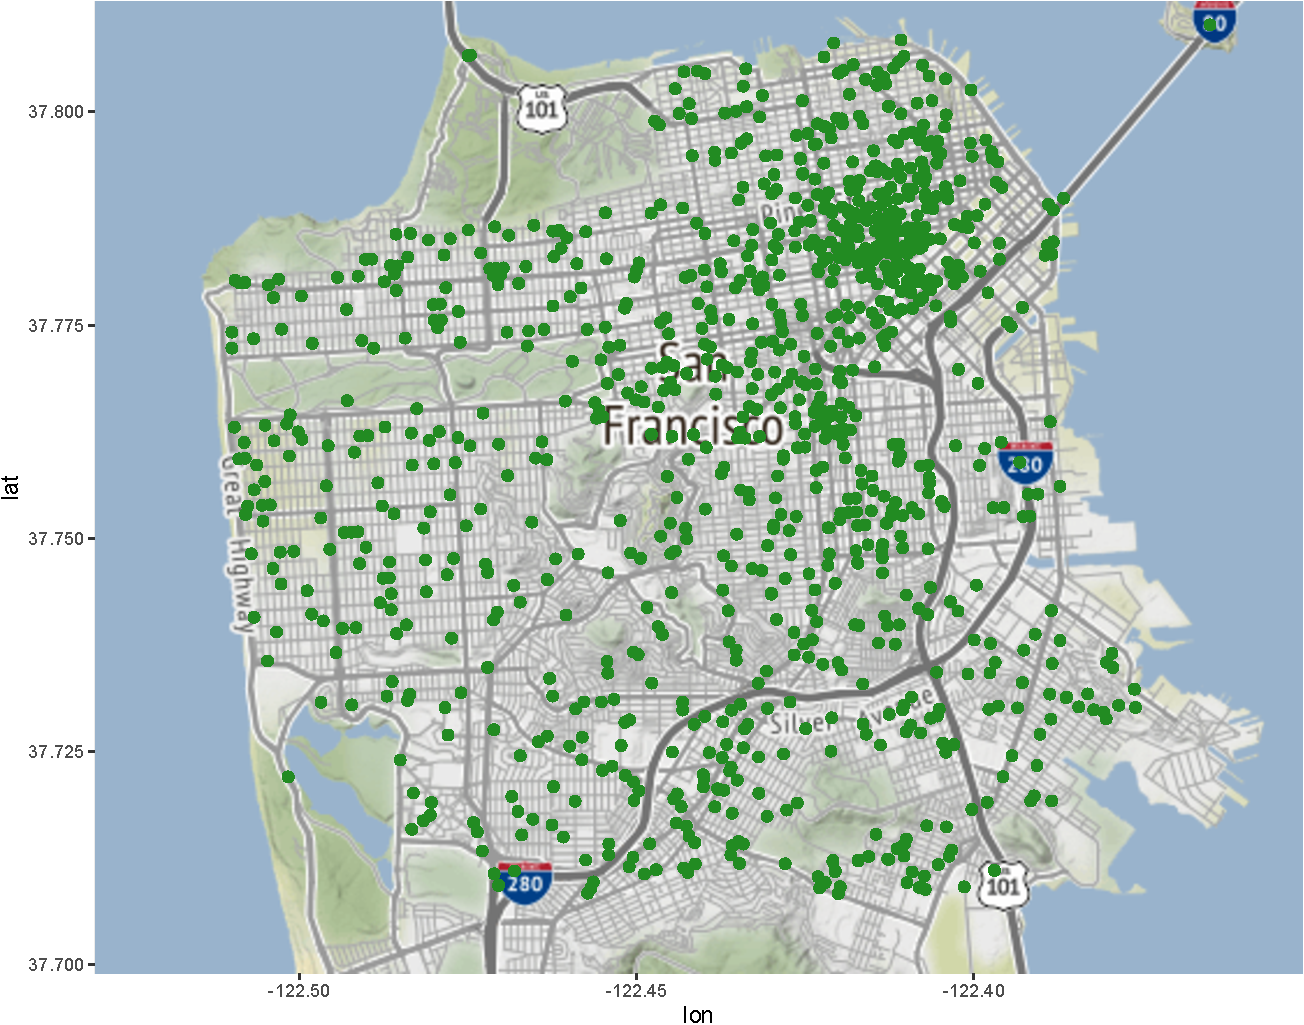
\includegraphics[width=1\linewidth,height=0.45\textheight,]{crimebythenumbers_files/figure-latex/unnamed-chunk-85-1} \end{center}

Most points are within a very narrow range so it appears
that our geocoding worked properly.

  \bibliography{book.bib}

\backmatter
\printindex

\end{document}
